% !TEX program = xelatex
\documentclass[UTF8,fontset=fandol,a4paper,11pt]{ctexart}
\usepackage[margin=21mm,top=23mm,bottom=22mm,headheight=16pt]{geometry}
\usepackage{amsmath,amssymb,mathtools,bm}
\usepackage{tikz}
\usetikzlibrary{arrows.meta,calc,angles,quotes,patterns}
\usepackage{xcolor,booktabs,array,longtable,enumitem,fancyhdr,needspace}
\usepackage[unicode,hidelinks]{hyperref}
\definecolor{ink}{HTML}{24343C}
\definecolor{accent}{HTML}{166A70}
\definecolor{muted}{HTML}{65747A}
\definecolor{rulegray}{HTML}{D4DDE0}
\definecolor{warm}{HTML}{966037}
\color{ink}
\setlength{\parindent}{2em}
\setlength{\parskip}{4pt}
\linespread{1.12}
\AtBeginDocument{\setlength{\abovedisplayskip}{6pt plus 2pt minus 1pt}
\setlength{\belowdisplayskip}{6pt plus 2pt minus 1pt}
\setlength{\abovedisplayshortskip}{0pt plus 1pt}
\setlength{\belowdisplayshortskip}{4pt plus 1pt}}
\setlist[enumerate]{label=(\arabic*),leftmargin=2.3em,itemsep=3pt,topsep=4pt}
\setlist[itemize]{leftmargin=2em,itemsep=2pt,topsep=4pt}
\allowdisplaybreaks[1]
\setlength{\emergencystretch}{2em}
\setcounter{secnumdepth}{0}
\providecommand{\tightlist}{\setlength{\itemsep}{0pt}\setlength{\parskip}{0pt}}
\ctexset{section={format=\Large\bfseries\color{accent},beforeskip=10pt,afterskip=9pt},
subsection={format=\normalsize\bfseries\color{accent},beforeskip=10pt,afterskip=4pt},
subsubsection={format=\normalsize\bfseries,beforeskip=8pt,afterskip=3pt}}
\pagestyle{fancy}
\fancyhf{}
\fancyhead[L]{\small\color{muted}物理学难题集萃}
% 页眉仅保留书名；版本名称只在封面显示。
\fancyfoot[L]{\small\color{muted}\chapterlabel}
\fancyfoot[R]{\small\thepage}
\renewcommand{\headrulewidth}{0.4pt}
\renewcommand{\footrulewidth}{0pt}
\newcommand{\dd}{\mathop{}\!\mathrm{d}}
\newcommand{\vect}[1]{\bm{#1}}
\newcommand{\tagline}[1]{\noindent{\small\color{muted}#1}\par}
\newcommand{\result}[1]{\begin{equation*}\boxed{#1}\end{equation*}}
\newcommand{\figcaption}[1]{\par\vspace{2pt}{\small\color{muted}#1}\par}
\newcommand{\teach}[2]{\Needspace{4\baselineskip}\subsection*{讲解要点与追问}#1\par\smallskip\noindent\textbf{追问：}#2\par}
\newcommand{\workarea}{\par\vspace{7mm}\noindent{\small\color{muted}作答区}\par\vspace{4mm}
\noindent\textcolor{rulegray}{\rule{\linewidth}{0.3pt}}\par\vspace{16mm}
\noindent\textcolor{rulegray}{\rule{\linewidth}{0.3pt}}\par\vspace{16mm}
\noindent\textcolor{rulegray}{\rule{\linewidth}{0.3pt}}\par\vspace{16mm}
\noindent\textcolor{rulegray}{\rule{\linewidth}{0.3pt}}}
\tikzset{axis/.style={-{Stealth[length=2mm]},thin,color=muted},
motion/.style={-{Stealth[length=2.3mm]},thick,color=accent},
force/.style={-{Stealth[length=2.3mm]},thick,color=warm},
traj/.style={thick,color=accent},guide/.style={dashed,thin,color=muted},
object/.style={thick,color=ink},every node/.style={font=\small}}\widowpenalty=10000\clubpenalty=10000\displaywidowpenalty=10000\newcommand{\chapterlabel}{光学试题}







\hypersetup{pdftitle={光学试题·学生解答版},pdfauthor={}}

\begin{document}\pdfbookmark[0]{光学试题}{cover}

\thispagestyle{empty}\vspace*{22mm}

\noindent{\Huge\bfseries 物理学难题集萃}\par\vspace{12mm}

\noindent{\LARGE 光学试题}\par\vspace{12mm}

\noindent{\Large\color{accent}学生解答版}\par\vspace{9mm}

\noindent\textcolor{accent}{\rule{\linewidth}{1pt}}\par\vspace{9mm}

\noindent 第1--6题\par\vfill\clearpage

\pdfbookmark[1]{题目目录}{contents}\section*{题目目录}

\begin{longtable}{@{}r p{113mm} r@{}}\toprule 题号 & 题目 & 页码\\\midrule

\hyperref[q:1]{1} & \hyperref[q:1]{有限共轭点的无像差凹面反射镜} & \pageref{q:1} \\

\hyperref[q:2]{2} & \hyperref[q:2]{双透镜成像与中间像处的场镜} & \pageref{q:2} \\

\hyperref[q:3]{3} & \hyperref[q:3]{惠更斯与冉斯登目镜的主点和焦点} & \pageref{q:3} \\

\hyperref[q:4]{4} & \hyperref[q:4]{切接透镜的干涉条纹与有限重叠区} & \pageref{q:4} \\

\hyperref[q:5]{5} & \hyperref[q:5]{双层膜三束反射光的相消与最薄组合} & \pageref{q:5} \\

\hyperref[q:6]{6} & \hyperref[q:6]{棱镜色散与衍射限制的分辨本领} & \pageref{q:6} \\

\bottomrule\end{longtable}

\clearpage

\pdfbookmark[2]{第 1 题 有限共轭点的无像差凹面反射镜}{q1}

\section*{第 1 题\quad 有限共轭点的无像差凹面反射镜}\label{q:1}


凹面反射镜顶点为$O$，轴上物点$Q$与$O$距离为$s>0$，要求从$Q$出发、落在反射面上的光线经一次反射后均会聚于轴上$Q'$；$Q'$与$O$距离为$s'>0$，两点在顶点同侧。反射面连通、光滑并包含顶点附近的一片区域，周围介质均匀。

以$O$为坐标原点、由物点一侧指向顶点的方向为$+x$，取$Q=(-s,0)$、$Q'=(-s',0)$。根据费马原理求子午截线方程、中心、长短半轴，并写出旋转曲面的方程；说明所得面为何满足反射定律。


\begin{center}\begin{minipage}{.98\linewidth}\centering
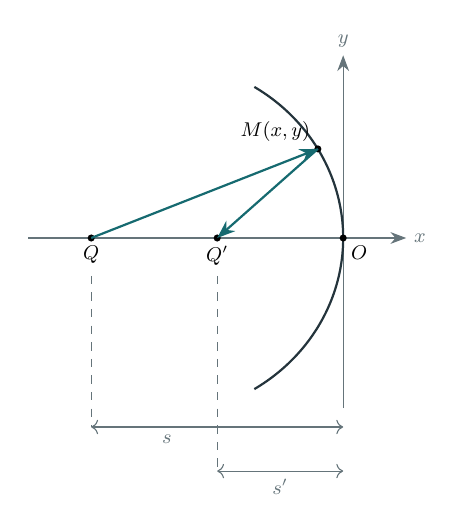
\begin{tikzpicture}[scale=.8,transform shape]

\draw[axis] (-5,0)--(1,0) node[right] {$x$};
\draw[axis] (0,-2.7)--(0,2.9) node[above] {$y$};
\draw[object,domain=-58:58,samples=100] plot ({-3+3*cos(\x)},{2.828427*sin(\x)});
\coordinate (Q) at (-4,0);\coordinate (V) at (-2,0);\coordinate (M) at (-.401924,1.414214);
\fill (Q) circle (1.6pt) node[below] {$Q$};
\fill (V) circle (1.6pt) node[below] {$Q'$};
\fill (0,0) circle (1.6pt) node[below right] {$O$};
\fill (M) circle (1.6pt) node[above left] {$M(x,y)$};
\draw[motion] (Q)--(M);\draw[motion] (M)--(V);
\draw[guide] (-4,-.6)--(-4,-3);\draw[guide] (-2,-.6)--(-2,-3.7);
\draw[axis,<->] (-4,-3)--(0,-3) node[pos=.3,below] {$s$};
\draw[axis,<->] (-2,-3.7)--(0,-3.7) node[midway,below] {$s'$};

\end{tikzpicture}
\figcaption{图光试.1\quad 两有限共轭点在顶点同侧，落到凹面上的光线反射后会聚。}
\end{minipage}\end{center}

\Needspace{6\baselineskip}\subsection*{解答}


图光试.1取反射点$M=(x,y)$。均匀介质中的光程与几何路程成正比，略去公共折射率，令
\[
\mathcal L(M)=|QM|+|MQ'|
=\sqrt{(x+s)^2+y^2}+\sqrt{(x+s')^2+y^2}.
\]
费马原理要求光线在反射点沿镜面的微小移动不改变一阶光程，即对任一镜面切向位移$d\boldsymbol r$有
$d\mathcal L=\nabla\mathcal L\cdot d\boldsymbol r=0$。因镜面连通，$\mathcal L$在这片反射面上为常量。顶点$O$给出常量$s+s'$，故
\[
\boxed{\sqrt{(x+s)^2+y^2}+\sqrt{(x+s')^2+y^2}=s+s'}.
\]
\begin{center}\begin{minipage}{.98\linewidth}\centering
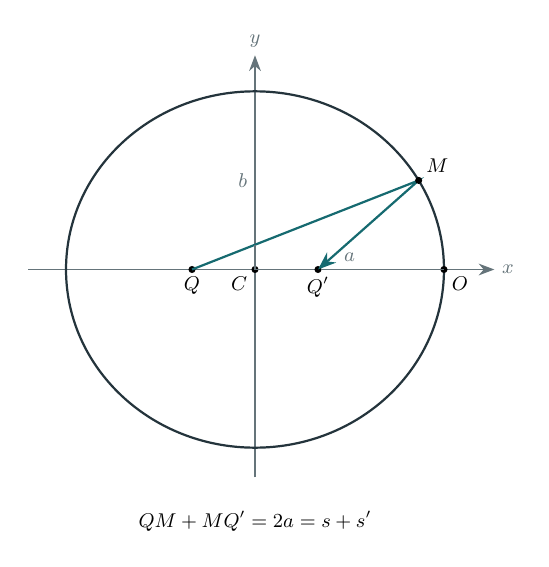
\begin{tikzpicture}[scale=.8,transform shape]

\draw[axis] (-6.6,0)--(.8,0) node[right] {$x$};
\draw[axis] (-3,-3.3)--(-3,3.4) node[above] {$y$};
\draw[object] (-3,0) ellipse (3 and 2.828427);
\fill (-4,0) circle (1.6pt) node[below] {$Q$};
\fill (-2,0) circle (1.6pt) node[below] {$Q'$};
\fill (-3,0) circle (1.6pt) node[below left] {$C$};
\fill (0,0) circle (1.6pt) node[below right] {$O$};
\draw[motion] (-4,0)--(-.401924,1.414214)--(-2,0);
\fill (-.401924,1.414214) circle (1.6pt) node[above right] {$M$};
\draw[guide] (-3,0)--(-3,2.828427) node[midway,left] {$b$};
\draw[guide] (-3,0)--(0,0) node[midway,above] {$a$};
\node at (-3,-4) {$QM+MQ'=2a=s+s'$};

\end{tikzpicture}
\figcaption{解图光试.1A\quad 双焦点定义给出椭圆中心与半轴，右端顶点为O。}
\end{minipage}\end{center}
解图光试.1A中两条焦径之和为$2a=s+s'$。为把几何条件化成直角坐标方程，记$D=s+s'$、$\eta=(s-s')/D$，先移项一次平方：
\[
\begin{aligned}
(x+s)^2+y^2
&=D^2+(x+s')^2+y^2
-2D\sqrt{(x+s')^2+y^2},\\
(s-s')x&=s'D-D\sqrt{(x+s')^2+y^2},\\
\sqrt{(x+s')^2+y^2}&=s'-\eta x.
\end{aligned}
\]
再平方并整理，
\[
(x+s')^2+y^2=(s'-\eta x)^2,
\]
\[
\frac{4ss'}{D^2}x^2+\frac{4ss'}D x+y^2=0.
\]
先除以$4ss'$，再将$x$的线性项配成平方：
\[
\frac{x^2}{D^2}+\frac{x}{D}+\frac{y^2}{4ss'}=0,
\qquad
\left(\frac{x}{D}+\frac12\right)^2+\frac{y^2}{4ss'}=\frac14.
\]
乘回$D^2$，即$(x+D/2)^2+D^2y^2/(4ss')=D^2/4$，因而得到
\[
\boxed{\frac{(x+D/2)^2}{(D/2)^2}+\frac{y^2}{ss'}=1}.
\]
所以截线为椭圆，中心和半轴分别为
\[
\boxed{C=(-D/2,0),\qquad a=D/2,\qquad b=\sqrt{ss'}}.
\]
由$a^2-b^2=(s-s')^2/4$，焦距半长$c=|s-s'|/2$，两个焦点恰为$Q,Q'$。椭圆上$-D\le x\le0$，而未平方关系中的
$s'-\eta x$在两端分别为$s$和$s'$，全段非负，因此整个椭圆都满足两段距离之和为$D$。所用凹镜取椭圆靠近$O$的一段，三维取对应的旋转面片。
\begin{center}\begin{minipage}{.98\linewidth}\centering
\begin{tikzpicture}[scale=.8,transform shape]

\draw[axis] (-5,0)--(1,0) node[right] {$x$};
\draw[axis] (0,-2.7)--(0,2.9) node[above] {$y$};
\draw[object,domain=-58:58,samples=100] plot ({-3+3*cos(\x)},{2.828427*sin(\x)});
\coordinate (Q) at (-4,0);\coordinate (V) at (-2,0);\coordinate (M) at (-.401924,1.414214);
\fill (Q) circle (1.6pt) node[below] {$Q$};
\fill (V) circle (1.6pt) node[below] {$Q'$};
\fill (0,0) circle (1.6pt) node[below right] {$O$};
\fill (M) circle (1.6pt) node[above left] {$M(x,y)$};
\draw[motion] (Q)--(M);\draw[motion] (M)--(V);
\draw[guide] (-4,-.6)--(-4,-3);\draw[guide] (-2,-.6)--(-2,-3.7);
\draw[axis,<->] (-4,-3)--(0,-3) node[pos=.3,below] {$s$};
\draw[axis,<->] (-2,-3.7)--(0,-3.7) node[midway,below] {$s'$};

\draw[force] (-1.4,.802)--(.95,2.243) node[right] {$\boldsymbol n$};
\draw[guide] (-.9,2.23)--(.1,.59);
\node[align=left] at (-4.5,3.5) {$\boldsymbol n\parallel\boldsymbol u_{\rm in}-\boldsymbol u_{\rm out}$\\两光线切向分量相同};

\end{tikzpicture}
\figcaption{解图光试.1B\quad 距离和梯度为镜面法向，反射光从M指向像点。}
\end{minipage}\end{center}
解图光试.1B中，入射单位向量为
$\boldsymbol u_{\rm in}=(M-Q)/|M-Q|$，反射后指向$Q'$的单位向量为
$\boldsymbol u_{\rm out}=(Q'-M)/|Q'-M|$。距离和的梯度
\[
\nabla\mathcal L=\boldsymbol u_{\rm in}-\boldsymbol u_{\rm out}
\]
沿镜面法向，所以两条射线的切向分量相同。在线段 $QQ^\prime$ 上，两段距离的和为 $|s-s^\prime|<D$。这个线段包含距离梯度可能相消的全部位置。镜面上两段距离和为 $D$，因此 $\nabla\mathcal L$ 给出非零法向。两个单位方向彼此不同，模均为1、切向分量相同。由单位长度关系，两者法向分量的平方相等；彼此不同又使其法向分量取相反号，因而给出入射角等于反射角。反射方向因而由$M$指向$Q'$。

三维情况下只将$y^2$换成$y^2+z^2$：
\[
\boxed{\frac{(x+D/2)^2}{(D/2)^2}+\frac{y^2+z^2}{ss'}=1}.
\]
距离和本身对$x$轴旋转不变，因而得到旋转椭球面。若$s=s'$，则$a=b=s$，曲面成为以$Q=Q'$为中心的球面，光线沿径向反射返回。


\Needspace{13\baselineskip}

\pdfbookmark[2]{第 2 题 双透镜成像与中间像处的场镜}{q2}

\section*{第 2 题\quad 双透镜成像与中间像处的场镜}\label{q:2}


沿光轴依次放置两块会聚薄透镜$L_1,L_2$，焦距均为$10\,\mathrm{cm}$，间距$70\,\mathrm{cm}$。物在$L_1$前$20\,\mathrm{cm}$处。
\begin{enumerate}
\item 求最后像的位置、横向放大率及正倒。
\item 在两镜之间增加有限正焦距薄透镜$L_3$，使最后像的位置仍保持不变，确定其位置。
\item 结合特殊光线说明$L_3$怎样使一部分被$L_2$孔径挡住的离轴光重新参与成像；说明增加透镜的集光作用所需的孔径条件。
\end{enumerate}
采用傍轴近似，忽略透镜吸收；分别讨论最后像的位置和孔径传光量。


\begin{center}\begin{minipage}{.98\linewidth}\centering
\begin{tikzpicture}[scale=.8,transform shape]

\draw[axis] (-2.8,0)--(9,0) node[right] {$x$};
\draw[object,<->] (0,-1.8)--(0,1.8) node[above] {$L_1,\ f_1=10\,\mathrm{cm}$};
\draw[object,<->] (7,-1.8)--(7,1.8) node[above] {$L_2,\ f_2=10\,\mathrm{cm}$};
\draw[motion] (-2,0)--(-2,.6) node[above] {物};
\draw[axis,<->] (-2,-1)--(0,-1) node[midway,below] {$20\,\mathrm{cm}$};
\draw[axis,<->] (0,-2.2)--(7,-2.2) node[midway,below] {$70\,\mathrm{cm}$};

\end{tikzpicture}
\figcaption{图光试.2\quad 两会聚透镜的已知焦距、间距与物距。}
\end{minipage}\end{center}

\Needspace{6\baselineskip}\subsection*{解答}


图光试.2以$L_1$为$x=0$、$L_2$为$x=70\,\mathrm{cm}$，光向右传播。第一块透镜的物距$s_1=20\,\mathrm{cm}$，由
\[
\frac1{s_1}+\frac1{s'_1}=\frac1{f_1}
\]
得$s'_1=20\,\mathrm{cm}$，中间像$I_1$位于$x=20\,\mathrm{cm}$，放大率$m_1=-s'_1/s_1=-1$。

对$L_2$，物距为$s_2=70-20=50\,\mathrm{cm}$，故
\[
s'_2=\frac{f_2s_2}{s_2-f_2}
=\frac{10\times50}{50-10}=12.5\,\mathrm{cm},
\qquad m_2=-\frac{12.5}{50}=-\frac14.
\]
因此最后像$I_2$在$L_2$后$12.5\,\mathrm{cm}$、即$x=82.5\,\mathrm{cm}$，且
\[
\boxed{m=m_1m_2=\frac14}.
\]
它是正立、缩小的实像，两次倒立相互抵消。
\begin{center}\begin{minipage}{.98\linewidth}\centering
\begin{tikzpicture}[scale=.8,transform shape]

\draw[axis] (-2.8,0)--(9,0) node[right] {$x$};
\draw[object,<->] (0,-1.8)--(0,1.8) node[above] {$L_1$};
\draw[object,<->] (7,-1.8)--(7,1.8) node[above] {$L_2$};
\draw[motion] (-2,0)--(-2,.6) node[above] {物};
\node[below left] at (2,-.2) {$I_1$};
\draw[guide] (8.25,-1.2)--(8.25,1.2) node[above] {$I_2$};
\foreach \x/\v in {-2/-20,0/0,2/20,7/70,8.25/82.5}{\node[below] at (\x,-1.9) {$\v$};}
\node at (3.5,-2.7) {坐标单位：$\mathrm{cm}$};

\draw[object,<->] (2,-1.5)--(2,1.5) node[above] {$L_3$};
\draw[traj] (-2,.2)--(0,.3)--(2,-.2)--(7,-.75)--(8.25,.05);
\draw[force] (-2,.2)--(0,-.3)--(2,-.2)--(7,.75)--(8.25,.05);
\fill (2,-.2) circle (1.6pt);\fill (8.25,.05) circle (1.6pt);

\end{tikzpicture}
\figcaption{解图光试.2A\quad L3在中间像平面，改变离轴交点后的斜率，最后像面保持不变。}
\end{minipage}\end{center}
解图光试.2A中同一物点的各条光线在$I_1$交于同一点。把$L_3$放在该中间像平面，只会改变光线的斜率，不改变交点高度；$L_2$所“看到”的物点仍是$I_1$，所以最后像面和横向倍率不变：
\[
\boxed{x_{L_3}=20\,\mathrm{cm}\quad\text{即距}L_2\text{为}50\,\mathrm{cm}}.
\]
再用成像矩阵求镜间其余位置的作用。用光线列向量$(y,\vartheta)^\mathsf T$，
\[
P(d)=\begin{pmatrix}1&d\\0&1\end{pmatrix},\qquad
K(f)=\begin{pmatrix}1&0\\-1/f&1\end{pmatrix}.
\]
保持原物面与最后像面不变，在$x$处插入$L_3$后，成像矩阵中的$B$元改变量为
\[
\Delta B=-\frac{B_{\rm after}B_{\rm before}}{f_3}.
\]
由$P(x)K(10)P(20)$得到$B_{\rm before}=20-x$；由
$P(12.5)K(10)P(70-x)$得到$B_{\rm after}=(x-20)/4$。所以
\[
\Delta B=\frac{(x-20)^2}{4f_3}.
\]
有限$f_3>0$时，要使$\Delta B=0$，在两镜间只有$x=20\,\mathrm{cm}$。这里的矩阵距离与焦距均以厘米计，$B$元的量纲为长度。
\begin{center}\begin{minipage}{.98\linewidth}\centering
\begin{tikzpicture}[scale=.7,transform shape]

\node at (3.1,2) {未加场镜：一条边缘光线被第二镜挡住};
\draw[axis] (-2.7,0)--(8.7,0);
\draw[object,<->] (0,-1.2)--(0,1.2) node[above] {$L_1$};
\draw[object,line width=1.3pt] (7,-1)--(7,1) node[above] {$L_2$};
\draw[guide] (7,-2.5)--(7,-1);
\draw[traj] (-2,.4)--(0,.35)--(2,-.4)--(7,-2.275);
\draw[force] (-2,.4)--(0,-.35)--(2,-.4)--(7,-.525)--(8.25,.1);
\node[right] at (7,-2.275) {遮挡};
\fill (2,-.4) circle (1.6pt) node[below] {$I_1$};
\begin{scope}[yshift=-6cm]
\node at (3.1,2) {加入场镜：将第一镜孔径成像到第二镜};
\draw[axis] (-2.7,0)--(8.7,0);
\draw[object,<->] (0,-1.2)--(0,1.2) node[above] {$L_1$};
\draw[object,<->] (2,-1.2)--(2,1.2) node[above] {$L_3$};
\draw[object,line width=1.3pt] (7,-1)--(7,1) node[above] {$L_2$};
\draw[traj] (-2,.4)--(0,.35)--(2,-.4)--(7,-.875)--(8.25,.1);
\draw[force] (-2,.4)--(0,-.35)--(2,-.4)--(7,.875)--(8.25,.1);
\fill (2,-.4) circle (1.6pt);\fill (8.25,.1) circle (1.6pt) node[above right] {$I_2$};
\node at (3,-2) {$f_3=100/7\,\mathrm{cm},\qquad y_{L_2}=-2.5h$};
\end{scope}

\end{tikzpicture}
\figcaption{解图光试.2B\quad 同一离轴点、同一第一镜入射孔径，比较第二镜处的截取。}
\end{minipage}\end{center}
解图光试.2B比较同一离轴点在加入场镜前后的光束。场镜位于中间像面，改变的是该点光锥的朝向；若$L_2$原先截去其中一部分，适当选择$f_3$可让更多光落入$L_2$有效孔径。参与成像的光先通过$L_1$，场镜自身口径也应容纳这些光线在中间像面的交点。

设物点高度为$y_0$，光线通过$L_1$时高度为$h$。从物点到$L_1$的斜率为$(h-y_0)/20$，经$L_1$后
\[
\vartheta_1=\frac{h-y_0}{20}-\frac h{10}
=-\frac{h+y_0}{20}.
\]
在中间像面$y_{I_1}=h+20\vartheta_1=-y_0$；通过场镜后
$\vartheta_3=\vartheta_1+y_0/f_3$。到$L_2$时
\[
\boxed{y_{L_2}=-\frac52h+
\left(-\frac72+\frac{50}{f_3}\right)y_0}.
\]
不加场镜时，离轴光束中心偏移$-7y_0/2$。例如取
$f_3=100/7\,\mathrm{cm}$，该偏移项消失，$L_1$的孔径平面也恰由$L_3$成像到$L_2$，使离轴光束更便于进入第二块透镜。设三个透镜的有效半径为 $R_1,R_2,R_3$。在解图光试.2B 的纵截面内，对第一镜边缘 $h=\pm R_1$ 代入上式，得第二镜处的光锥半宽为 $5R_1/2$，中心高度为 $(-7/2+50/f_3)y_0$。要使第一镜收集的这束光全部通过，需满足
\[
|y_0|\le R_3,\qquad
\frac52R_1+\left|\left(-\frac72+\frac{50\,\mathrm{cm}}{f_3}\right)y_0\right|\le R_2 .
\]
前式保证场镜容纳中间像点，后式保证第二镜容纳光锥的两侧外缘。取 $f_3=100/7\,\mathrm{cm}$ 时，光锥中心与第二镜光心重合，因此全束通过要求 $R_2\ge5R_1/2$。第二镜在加场镜前已接收全束时，该选择保持通光量；原来只接收部分光束时，图 B 给出重新利用其余部分的条件。

用特殊光线也可直接作图。解图光试.2C取离轴物点$P$，$PM$平行主轴，$PN$经过第一镜光心。经$L_1$后，$PM$通过第一镜后焦点，$PN$保持直线，二者交于$I_1$。它们经$I_1$后在第二镜处的高度，正是上式分别代入$h=y_0$与$h=0$所得：未加场镜时为$-6y_0$与$-3.5y_0$，取$f_3=100/7\,\mathrm{cm}$后为$-2.5y_0$与$0$。因此，落在较低处而被第二镜孔径截去的这部分光束可以转入有效孔径，继续在同一$I_2$会聚。
\begin{center}\begin{minipage}{.98\linewidth}\centering
\begin{tikzpicture}[scale=0.8,transform shape]
\draw[axis] (0,0)--(9.2,0);\draw[axis] (0,0)--(0,3.8000000000000003);
\draw[thin,color=muted] (0.2488479,0)--(0.2488479,-.07);\node[below] at (0.2488479,-.09) {$-20$};
\draw[thin,color=muted] (1.9078341,0)--(1.9078341,-.07);\node[below] at (1.9078341,-.09) {$0$};
\draw[thin,color=muted] (3.5668203,0)--(3.5668203,-.07);\node[below] at (3.5668203,-.09) {$20$};
\draw[thin,color=muted] (7.7142857,0)--(7.7142857,-.07);\node[below] at (7.7142857,-.09) {$70$};
\draw[thin,color=muted] (0,2.4923077)--(-.07,2.4923077);\node[left] at (-.09,2.4923077) {$0$};
\node[below] at (4.5,-.64) {$x$（厘米）};\node[above right] at (0,3.85) {$y$（厘米）};
\draw[guide] (0,2.4923077)--(9.0,2.4923077);\draw[object,<->] (1.9078341,1.5230769)--(1.9078341,3.4615385) node[above] {$L_1$};\draw[object,<->] (7.7142857,1.5230769)--(7.7142857,3.4615385) node[above] {$L_2$};\draw[object,<->] (3.5668203,1.5230769)--(3.5668203,3.4615385) node[above] {$L_3$};\draw[traj] plot coordinates {(0.2488479,2.8615385) (1.9078341,2.8615385) (3.5668203,2.1230769) (7.7142857,1.5692308) (8.7511521,2.5846154)};
\draw[dashed,color=muted] plot coordinates {(3.5668203,2.1230769) (7.7142857,0.2769231)};
\draw[force] plot coordinates {(0.2488479,2.8615385) (1.9078341,2.4923077) (3.5668203,2.1230769) (7.7142857,2.4923077) (8.7511521,2.5846154)};
\draw[dashed,color=muted] plot coordinates {(3.5668203,2.1230769) (7.7142857,1.2000000)};
\fill (0.2488479,2.8615385) circle(.03) node[above left] {$P$};\fill (1.9078341,2.8615385) circle(.03) node[above left] {$M$};\fill (1.9078341,2.4923077) circle(.03) node[below left] {$N$};\fill (3.5668203,2.1230769) circle(.03) node[below] {$I_1$};\fill (8.7511521,2.5846154) circle(.03) node[right] {$I_2$};\end{tikzpicture}
\figcaption{解图光试.2C\quad 平行轴光线PM与过光心光线PN：虚线为未加场镜的延长线}
\end{minipage}\end{center}


\Needspace{13\baselineskip}

\pdfbookmark[2]{第 3 题 惠更斯与冉斯登目镜的主点和焦点}{q3}

\section*{第 3 题\quad 惠更斯与冉斯登目镜的主点和焦点}\label{q:3}


目镜由场镜$L_1$和接目镜$L_2$组成，两者均为会聚薄透镜，焦距分别为$f_1,f_2$，间距$d$，前后均为空气。光从左向右，取$L_1$位置为$x=0$、$L_2$为$x=d$。
\begin{enumerate}
\item 惠更斯目镜满足$f_1:f_2:d=3:1:2$；令$f_2=a$，求有效焦距、物方主点$H$、像方主点$H'$、物方焦点$F$及像方焦点$F'$的绝对坐标。
\item 冉斯登目镜满足$f_1:f_2:d=1:1:2/3$；令$f_1=f_2=a$，求相同各量。
\item 哪一种可将物体放在整组透镜之前，当作普通放大镜使用？结合物方焦点位置说明。
\end{enumerate}
采用傍轴近似，所有位置统一用向右为正的$x$坐标表达。


\begin{center}\begin{minipage}{.98\linewidth}\centering
\begin{tikzpicture}[scale=.85,transform shape]

\draw[axis] (-1,0)--(8,0) node[right] {$x$};
\draw[object,<->] (0,-1.5)--(0,1.5) node[above] {$L_1$};
\draw[object,<->] (6,-1.5)--(6,1.5) node[above] {$L_2$};
\node[below] at (0,-1.5) {$x=0$};\node[below] at (6,-1.5) {$x=d$};
\draw[axis,<->] (0,-2.5)--(6,-2.5) node[midway,below] {$d$};
\node at (3,2.6) {光从左向右；两侧介质均为空气};

\end{tikzpicture}
\figcaption{图光试.3\quad 先固定坐标，再计算组合系统的主点和焦点。}
\end{minipage}\end{center}

\Needspace{6\baselineskip}\subsection*{解答}


图光试.3中每片透镜有各自的焦点；整组主点和焦点由两次折射与镜间传播共同确定。

用传播矩阵$P(d)$和薄透镜矩阵$K(f)$表示，系统从$L_1$前到$L_2$后为
\[
\begin{aligned}
M&=K(f_2)P(d)K(f_1)\\
&=\begin{pmatrix}
1-d/f_1&d\\
-(f_1+f_2-d)/(f_1f_2)&1-d/f_2
\end{pmatrix}.
\end{aligned}
\]
记有效焦距为$f_{\rm e}$，有
\[
\boxed{f_{\rm e}=\frac{f_1f_2}{f_1+f_2-d}}.
\]
为了定位主点，把同一矩阵写成从$L_1$传播到$H$、经等效薄透镜、再从$H'$传播到$L_2$：
\[
M=P(q)K(f_{\rm e})P(p),\qquad
p=x_H,\quad q=d-x_{H'}.
\]
展开右式的对角元为$1-q/f_{\rm e}$、$1-p/f_{\rm e}$。逐项比较得
\[
\boxed{x_H=\frac{f_{\rm e}d}{f_2}},\qquad
\boxed{x_{H'}=d-\frac{f_{\rm e}d}{f_1}}.
\]
在同一空气介质中，前焦点位于$H$左方$f_{\rm e}$，后焦点位于$H'$右方$f_{\rm e}$，所以
\[
\boxed{x_F=x_H-f_{\rm e}},\qquad
\boxed{x_{F'}=x_{H'}+f_{\rm e}}.
\]
主点可落在两镜之外，矩阵中的形式传播长度也允许为负。该分解记录真实系统输入、输出光线之间的等效关系，实际传播仍依次通过两片透镜。
\begin{center}\begin{minipage}{.98\linewidth}\centering
\begin{tikzpicture}[scale=.8,transform shape]

\draw[axis] (-.8,0)--(10.5,0) node[right] {$x/a$};
\draw[object,<->] (0,-1.2)--(0,1.2) node[above] {$L_1$};
\draw[object,<->] (6,-1.2)--(6,1.2) node[above] {$L_2$};
\foreach \x/\v in {0/0,3/1,4.5/{3/2},6/2,7.5/{5/2},9/3}{\draw (\x,-.08)--(\x,.08);\node[below,fill=white,inner sep=1pt] at (\x,-.2) {$\v$};}
\draw[guide] (3,0)--(3,-1.5) node[below] {$H'$};
\draw[guide] (9,0)--(9,-1.5) node[below] {$H$};
\draw[guide] (4.5,0)--(4.5,1.6) node[above] {$F$};
\draw[guide] (7.5,0)--(7.5,1.6) node[above] {$F'$};
\draw[axis,<->] (3,2.8)--(7.5,2.8) node[midway,above] {$f_{\rm e}=3a/2$};
\draw[axis,<->] (4.5,-2.8)--(9,-2.8) node[midway,below] {$f_{\rm e}=3a/2$};
\node at (4.5,4) {惠更斯：前焦点在两镜之间};

\end{tikzpicture}
\figcaption{解图光试.3A\quad 有效焦距从主点量起，H在第二镜之后。}
\end{minipage}\end{center}
第（1）问取$f_1=3a,f_2=a,d=2a$。解图光试.3A按统一坐标标出结果：
\[
f_{\rm e}=\frac{3a^2}{3a+a-2a}=\frac32a,
\]
\[
x_H=3a,\qquad x_{H'}=2a-a=a,
\]
\[
\boxed{x_F=\frac32a,\qquad x_{F'}=\frac52a}.
\]
第一镜的像方焦点在$x=3a$，第二镜的像方焦点也在$x=2a+a=3a$，两者重合于物方主点$H$所在位置；第二镜的物方焦点则在$x=2a-a=a$，处于两镜正中。这些是单片透镜的焦点，整组焦点为上式的$3a/2$与$5a/2$。

因此$H$在第二镜后$a$处，$H'$在两镜正中；物方焦点$F$也在两镜之间，像方焦点$F'$在第二镜后$a/2$处。这里$H$位于$H'$右侧，两者名称由物方、像方等效关系确定。
\begin{center}\begin{minipage}{.98\linewidth}\centering
\begin{tikzpicture}[scale=.8,transform shape]

\draw[axis] (-2.5,0)--(7,0) node[right] {$x/a$};
\draw[object,<->] (0,-1.2)--(0,1.2) node[above] {$L_1$};
\draw[object,<->] (4,-1.2)--(4,1.2) node[above] {$L_2$};
\foreach \x/\v in {-1.5/{-1/4},0/0,1/{1/6},3/{1/2},4/{2/3},5.5/{11/12}}{\draw (\x,-.08)--(\x,.08);\node[below,fill=white,inner sep=1pt] at (\x,-.2) {$\v$};}
\draw[guide] (1,0)--(1,-1.6) node[below] {$H'$};
\draw[guide] (3,0)--(3,-1.6) node[below] {$H$};
\draw[guide] (-1.5,0)--(-1.5,1.7) node[above] {$F$};
\draw[guide] (5.5,0)--(5.5,1.7) node[above] {$F'$};
\draw[axis,<->] (1,2.9)--(5.5,2.9) node[midway,above] {$f_{\rm e}=3a/4$};
\draw[axis,<->] (-1.5,-2.9)--(3,-2.9) node[midway,below] {$f_{\rm e}=3a/4$};
\node at (2,4.1) {冉斯登：前焦点在整组之前};

\end{tikzpicture}
\figcaption{解图光试.3B\quad 两主点在镜间，实物可放在第一镜之前的前焦面附近。}
\end{minipage}\end{center}
第（2）问取$f_1=f_2=a,d=2a/3$。解图光试.3B给出
\[
f_{\rm e}=\frac{a^2}{2a-2a/3}=\frac34a,
\]
\[
x_H=\frac a2,\qquad
x_{H'}=\frac{2a}3-\frac a2=\frac a6,
\]
\[
\boxed{x_F=-\frac a4,\qquad x_{F'}=\frac{11a}{12}}.
\]
后焦点在$L_2$后$a/4$，前焦点在$L_1$前$a/4$。

解图光试.3C把两种焦点的光线定义画出：平行入射光经过惠更斯组合，在第二镜后$a/2$会聚；从冉斯登前焦面同一点发出的光经两镜后平行。第一条光路以第二镜处的高度与出射斜率求交点，第二条以同一物点的不同入射斜率说明平行出射，均与主面量取的有效焦距相接。
\begin{center}\begin{minipage}{.98\linewidth}\centering
\begin{tikzpicture}[scale=0.8,transform shape]
\draw[axis] (0,0)--(7.2,0);\draw[axis] (0,0)--(0,2.9000000000000004);
\draw[thin,color=muted] (1.2000000,0)--(1.2000000,-.07);\node[below] at (1.2000000,-.09) {$0$};
\draw[thin,color=muted] (5.2000000,0)--(5.2000000,-.07);\node[below] at (5.2000000,-.09) {$2$};
\draw[thin,color=muted] (0,1.3500000)--(-.07,1.3500000);\node[left] at (-.09,1.3500000) {$0$};
\node[below] at (3.5,-.64) {$x/a$};\node[above right] at (0,2.95) {$y/a$};
\draw[guide] (0,1.3500000)--(7.0,1.3500000);\draw[object,<->] (1.2000000,.1)--(1.2000000,2.6000000) node[above] {$L_1$};\draw[object,<->] (5.2000000,.1)--(5.2000000,2.6000000) node[above] {$L_2$};\draw[traj] plot coordinates {(0.4000000,1.9285714) (1.2000000,1.9285714) (5.2000000,1.5428571) (6.6000000,1.2728571)};
\draw[force] plot coordinates {(0.4000000,0.7714286) (1.2000000,0.7714286) (5.2000000,1.1571429) (6.6000000,1.4271429)};
\node[above] at (3.5,3.65) {惠更斯：平行入射光在$x/a=5/2$会聚};\begin{scope}[yshift=-7cm]\draw[axis] (0,0)--(7.2,0);\draw[axis] (0,0)--(0,2.9000000000000004);
\draw[thin,color=muted] (1.4000000,0)--(1.4000000,-.07);\node[below] at (1.4000000,-.09) {$0$};
\draw[thin,color=muted] (3.4740741,0)--(3.4740741,-.07);\node[below] at (3.4740741,-.09) {$0.6667$};
\draw[thin,color=muted] (0,1.3500000)--(-.07,1.3500000);\node[left] at (-.09,1.3500000) {$0$};
\node[below] at (3.5,-.64) {$x/a$};\node[above right] at (0,2.95) {$y/a$};
\draw[guide] (0,1.3500000)--(7.0,1.3500000);\draw[object,<->] (1.4000000,.1)--(1.4000000,2.6000000) node[above] {$L_1$};\draw[object,<->] (3.4740741,.1)--(3.4740741,2.6000000) node[above] {$L_2$};\draw[traj] plot coordinates {(0.6222222,1.4271429) (1.4000000,1.3885714) (3.4740741,1.2600000) (6.3777778,1.1640000)};
\draw[force] plot coordinates {(0.6222222,1.4271429) (1.4000000,1.4657143) (3.4740741,1.4914286) (6.3777778,1.3954286)};
\node[above] at (3.5,3.65) {冉斯登：物点在$x/a=-1/4$时平行出射};\end{scope}\end{tikzpicture}
\figcaption{解图光试.3C\quad 用实际光线分别定位后焦点与前焦面}
\end{minipage}\end{center}

第（3）问，普通放大镜需要把待观察实物放在整组之前、靠近前焦面，使出射光近于平行或形成较远虚像。冉斯登的前焦点在$x<0$，满足这一放置方式，所以可以作普通放大镜。惠更斯的前焦面在两镜之间，适于接收其他光学部件形成在镜间的中间像。对冉斯登，物点从 $x_F=-a/4$ 略向右移且仍位于第一镜之前时，从物方主点量出的物距满足 $0<s<f_{\rm e}$，出射光的反延线给出放大的正立虚像。对惠更斯，整组之前的实物从 $H$ 量起至少相距 $3a$，大于 $f_{\rm e}=3a/2$，按同一高斯式得到实像。


\Needspace{13\baselineskip}

\pdfbookmark[2]{第 4 题 切接透镜的干涉条纹与有限重叠区}{q4}

\section*{第 4 题\quad 切接透镜的干涉条纹与有限重叠区}\label{q:4}


一焦距$f=20\,\mathrm{cm}$的薄凸透镜，从中央切去宽为$a$的条带，再把剩下两半向中间平移并粘接。两半的光心相距$a$，粘接后的总直径为$D=2.0\,\mathrm{cm}$。波长$\lambda=500\,\mathrm{nm}$的单色点光源$S$位于粘接体的中心轴线上，距透镜为$f$。透镜另一侧放置垂直中心轴的屏，测得条纹间距$\Delta y=0.20\,\mathrm{mm}$。
\begin{enumerate}
\item 求切去条带的宽度$a$。
\item 屏距透镜多远时，可见重叠区内的条纹数最多？给出中央纵截面内重叠宽度随屏距的变化。
\end{enumerate}
采用傍轴几何光学描述光束外缘，在两束的重叠区域计算干涉；忽略边缘衍射对外缘的模糊。


\begin{center}\begin{minipage}{.98\linewidth}\centering
\begin{tikzpicture}[scale=.7,transform shape]

\draw[object] (-1,1.9)..controls(-1.8,.5)and(-1.8,-.5)..(-1,-1.9);
\draw[object] (-1,1.9)..controls(-.2,.5)and(-.2,-.5)..(-1,-1.9);
\fill[white] (-1.9,-.4) rectangle (-.1,.4);
\draw[guide] (-1.65,.4)--(-.35,.4);\draw[guide] (-1.65,-.4)--(-.35,-.4);
\draw[axis,<->] (-2.2,-.4)--(-2.2,.4) node[midway,left] {$a$};
\draw[motion] (0,0)--(1,0);
\draw[object] (2,1.5)..controls(1.3,.3)and(1.3,-.3)..(2,-1.5);
\draw[object] (2,1.5)..controls(2.7,.3)and(2.7,-.3)..(2,-1.5);
\draw[object] (1.5,0)--(2.5,0);
\draw[axis,<->] (3,-1.5)--(3,1.5) node[midway,right,yshift=4pt] {$D$};
\begin{scope}[xshift=6cm]
\draw[axis] (-2.5,0)--(3.5,0);
\fill (-2,0) circle (1.8pt) node[above] {$S$};
\draw[object,<->] (0,-1.5)--(0,1.5);
\draw[object] (3,-2)--(3,2) node[above] {屏};
\draw[axis,<->] (-2,-2.3)--(0,-2.3) node[midway,below] {$f$};
\draw[axis,<->] (0,-2.9)--(3,-2.9) node[midway,below] {$z$};
\end{scope}

\end{tikzpicture}
\figcaption{图光试.4\quad 中央去条带后平移粘接，D指粘接后的总口径。}
\end{minipage}\end{center}

\Needspace{6\baselineskip}\subsection*{解答}


图光试.4中，上半镜向下平移$a/2$，其光轴在中心轴下方$a/2$；下半镜则相反。光源虽在粘接体中心轴上，却分别位于两片光轴的两侧，并处于各片前焦平面。
\begin{center}\begin{minipage}{.98\linewidth}\centering
\begin{tikzpicture}[scale=.7,transform shape]

\fill[accent!12] (0,0)--(4,1)--(8,0)--(4,-1)--cycle;
\draw[axis] (-3,0)--(9,0) node[right] {$z$};
\draw[object] (0,-2)--(0,2);
\draw[traj] (0,0)--(8,-2);\draw[traj] (0,2)--(8,0);
\draw[force] (0,-2)--(8,0);\draw[force] (0,0)--(8,2);
\draw[guide] (0,-.4)--(3,-.4);
\draw[guide] (0,.4)--(3,.4);
\node at (4,3.2) {上半镜轴$y=-a/2$；下半镜轴$y=+a/2$};
\fill (-1.6,0) circle (1.8pt) node[above] {$S$};
\draw[guide] (-1.6,0)--(0,-.4);\draw[guide] (-1.6,0)--(0,.4);
\draw[axis,<->] (-.8,-.4)--(-.8,.4) node[midway,left] {$a$};
\draw[object] (4,-2)--(4,2) node[above] {示例屏};
\draw[motion] (1,1.7)--(2,1.45) node[midway,above] {$-\theta$};
\draw[motion] (1,-1.7)--(2,-1.45) node[midway,below] {$+\theta$};
\node at (4,-3) {两束均为平面波，阴影为中央纵截面的重叠区};

\end{tikzpicture}
\figcaption{解图光试.4A\quad 光轴偏移决定向内倾角，光束外缘由半孔径分别平移。}
\end{minipage}\end{center}
解图光试.4A中，每半镜把来自$S$的球面波变为平面波。上半束向下、下半束向上，两束方向相对中心轴为$-\theta,+\theta$。以$y$轴向上、$z$轴向右表示传播。薄透镜的傍轴折射关系为$u_{\rm out}=u_{\rm in}-(y-y_c)/f$，轴上焦面点发出的光在透镜处有$u_{\rm in}=y/f$，所以$u_{\rm out}=y_c/f$，与落点$y$无关。两半镜的光心坐标$y_c=\mp a/2$直接给出两个相反斜率。傍轴下
\[
\theta\simeq\frac{a}{2f}.
\]
在屏上取纵向坐标$y$，两平面波的波矢纵分量差为$2k\sin\theta$，相位差随$y$变化为
\[
\Delta\varphi(y)=2k\,y\sin\theta+\varphi_0.
\]
相位差由$({\boldsymbol k}_2-{\boldsymbol k}_1)\cdot(0,y,z)$给出，两束的纵向分量同为$k\cos\theta$，传播距离项抵消，只余横向的$2ky\sin\theta$。相邻亮纹相位差$2\pi$，所以
\[
\Delta y=\frac{\lambda}{2\sin\theta}
\simeq\frac{\lambda f}{a}.
\]
代入同一单位：
\[
\boxed{a=\frac{\lambda f}{\Delta y}
=\frac{(5.00\times10^{-7})(0.200)}{2.00\times10^{-4}}
=5.00\times10^{-4}\,\mathrm m=0.50\,\mathrm{mm}}.
\]
两束来自同一点光源并通过同一镜体的两部分，具有固定相位关系。常量$\varphi_0$会平移条纹，但不改变间距。
\begin{center}\begin{minipage}{.98\linewidth}\centering
\begin{tikzpicture}[scale=.8,transform shape]

\draw[axis] (0,0)--(9,0) node[right] {$z$};
\draw[axis] (0,0)--(0,3) node[above] {$W$};
\draw[traj] (0,0)--(4,2)--(8,0);
\draw[guide] (4,0)--(4,2)--(0,2);
\node[left] at (0,2) {$D/2$};
\node[below] at (4,0) {$D/(4\theta)$};
\node[below] at (8,0) {$D/(2\theta)$};
\node[above left] at (2,1.2) {$2z\theta$};
\node[above right] at (6,1.2) {$D-2z\theta$};
\node at (4.5,3.8) {条纹间距固定，重叠宽度决定间距数};

\end{tikzpicture}
\figcaption{解图光试.4B\quad 两段束边限制交替，最宽处对应最佳屏距。}
\end{minipage}\end{center}
第（2）问沿两束的内、外侧各追踪一条极限光线，共得到四条束边。解图光试.4B在中央纵截面中取透镜平面为$z=0$，屏为$z>0$。上、下半孔径分别覆盖$[0,D/2]$与$[-D/2,0]$。到屏上，上束整体向下移$z\theta$、下束向上移$z\theta$，区间变成
\[
\mathcal B_+(z)=[-z\theta,D/2-z\theta],\qquad
\mathcal B_-(z)=[-D/2+z\theta,z\theta].
\]
重叠区是这两个区间的交集。取上端点的较小值、下端点的较大值，宽度为
\[
W=\max\{0,\min(D/2-z\theta,z\theta)-\max(-z\theta,-D/2+z\theta)\}.
\]
两个候选上端点在$z\theta=D/4$相等，下端点也在同一位置交换大小；整理得到
\[
\boxed{W(z)=
\begin{cases}
2z\theta,&0\le z\le D/(4\theta),\\
D-2z\theta,&D/(4\theta)\le z\le D/(2\theta),\\
0,&z\ge D/(2\theta).
\end{cases}}
\]
开始时相邻内束边向对方孔径区域移动，宽度增加；超过中点后，外束边逐渐限制重叠，宽度反而减小。条纹间距与$z$无关，所以条纹总数在$W$最大时最多：
\[
\boxed{z_{\rm best}=\frac D{4\theta}
\simeq\frac{Df}{2a}
=\frac{0.0200\times0.200}{2\times0.000500}
=4.0\,\mathrm m}.
\]
此时$W_{\max}=D/2=1.0\,\mathrm{cm}$，覆盖约
$W_{\max}/\Delta y=50$ 个条纹间距。令 $\xi=\varphi_0/(2\pi)$。解图光试.4C 在 $4\,\mathrm m$ 处标出的两条束边夹住 $|y|<W_{\max}/2$，因此亮纹中心 $y_m=(m-\xi)\Delta y$ 对应
\[
\xi-25<m<\xi+25,\qquad
N_{\rm open}=\lceil \xi+25\rceil-\lfloor \xi-25\rfloor-1.
\]
若 $\xi$ 是整数，中心亮纹及其两侧各 $24$ 条落在开区间内，共 $49$ 条，两侧束边各恰有一个亮纹中心。两侧束边都计入时为 $51$ 条，只计一侧时为 $50$ 条。若 $\xi$ 不是整数，两侧束边都没有亮纹中心，区间内为 $50$ 条。光束边缘若计入衍射模糊，边缘亮纹能否辨认还取决于实际照度。这里的 $D$ 是粘接后的直径，上、下半孔径各高 $D/2$。
最佳屏上，两束区间均为$[-D/4,D/4]$，即它们的截面中心重合；四条束边在此将增长段接到下降段。继续传播到$z=D/(2\theta)$时，两区间仅在轴上接触，再向后分开。解图光试.4C按实际参数画出四条极限光线与$z=2,4,6\,\mathrm m$处的区间，显示三处的宽度依次为5、10、5毫米。
\begin{center}\begin{minipage}{.98\linewidth}\centering
\begin{tikzpicture}[scale=0.72,transform shape]
\draw[axis] (0,0)--(6.2,0);\draw[axis] (0,0)--(0,3.4000000000000004);
\draw[thin,color=muted] (0.0000000,0)--(0.0000000,-.07);\node[below] at (0.0000000,-.09) {$0$};
\draw[thin,color=muted] (1.5000000,0)--(1.5000000,-.07);\node[below] at (1.5000000,-.09) {$2$};
\draw[thin,color=muted] (3.0000000,0)--(3.0000000,-.07);\node[below] at (3.0000000,-.09) {$4$};
\draw[thin,color=muted] (4.5000000,0)--(4.5000000,-.07);\node[below] at (4.5000000,-.09) {$6$};
\draw[thin,color=muted] (6.0000000,0)--(6.0000000,-.07);\node[below] at (6.0000000,-.09) {$8$};
\draw[thin,color=muted] (0,0.0000000)--(-.07,0.0000000);\node[left] at (-.09,0.0000000) {$-10$};
\draw[thin,color=muted] (0,0.8000000)--(-.07,0.8000000);\node[left] at (-.09,0.8000000) {$-5$};
\draw[thin,color=muted] (0,1.6000000)--(-.07,1.6000000);\node[left] at (-.09,1.6000000) {$0$};
\draw[thin,color=muted] (0,2.4000000)--(-.07,2.4000000);\node[left] at (-.09,2.4000000) {$5$};
\draw[thin,color=muted] (0,3.2000000)--(-.07,3.2000000);\node[left] at (-.09,3.2000000) {$10$};
\node[anchor=west] at (6.32,0) {屏距$z$（米）};\node[above right] at (0,3.45) {束边$y$（毫米）};
\draw[traj] plot coordinates {(0.0000000,1.6000000) (0.0300000,1.5920000) (0.0600000,1.5840000) (0.0900000,1.5760000) (0.1200000,1.5680000) (0.1500000,1.5600000) (0.1800000,1.5520000) (0.2100000,1.5440000) (0.2400000,1.5360000) (0.2700000,1.5280000) (0.3000000,1.5200000) (0.3300000,1.5120000) (0.3600000,1.5040000) (0.3900000,1.4960000) (0.4200000,1.4880000) (0.4500000,1.4800000) (0.4800000,1.4720000) (0.5100000,1.4640000) (0.5400000,1.4560000) (0.5700000,1.4480000) (0.6000000,1.4400000) (0.6300000,1.4320000) (0.6600000,1.4240000) (0.6900000,1.4160000) (0.7200000,1.4080000) (0.7500000,1.4000000) (0.7800000,1.3920000) (0.8100000,1.3840000) (0.8400000,1.3760000) (0.8700000,1.3680000) (0.9000000,1.3600000) (0.9300000,1.3520000) (0.9600000,1.3440000) (0.9900000,1.3360000) (1.0200000,1.3280000) (1.0500000,1.3200000) (1.0800000,1.3120000) (1.1100000,1.3040000) (1.1400000,1.2960000) (1.1700000,1.2880000) (1.2000000,1.2800000) (1.2300000,1.2720000) (1.2600000,1.2640000) (1.2900000,1.2560000) (1.3200000,1.2480000) (1.3500000,1.2400000) (1.3800000,1.2320000) (1.4100000,1.2240000) (1.4400000,1.2160000) (1.4700000,1.2080000) (1.5000000,1.2000000) (1.5300000,1.1920000) (1.5600000,1.1840000) (1.5900000,1.1760000) (1.6200000,1.1680000) (1.6500000,1.1600000) (1.6800000,1.1520000) (1.7100000,1.1440000) (1.7400000,1.1360000) (1.7700000,1.1280000) (1.8000000,1.1200000) (1.8300000,1.1120000) (1.8600000,1.1040000) (1.8900000,1.0960000) (1.9200000,1.0880000) (1.9500000,1.0800000) (1.9800000,1.0720000) (2.0100000,1.0640000) (2.0400000,1.0560000) (2.0700000,1.0480000) (2.1000000,1.0400000) (2.1300000,1.0320000) (2.1600000,1.0240000) (2.1900000,1.0160000) (2.2200000,1.0080000) (2.2500000,1.0000000) (2.2800000,0.9920000) (2.3100000,0.9840000) (2.3400000,0.9760000) (2.3700000,0.9680000) (2.4000000,0.9600000) (2.4300000,0.9520000) (2.4600000,0.9440000) (2.4900000,0.9360000) (2.5200000,0.9280000) (2.5500000,0.9200000) (2.5800000,0.9120000) (2.6100000,0.9040000) (2.6400000,0.8960000) (2.6700000,0.8880000) (2.7000000,0.8800000) (2.7300000,0.8720000) (2.7600000,0.8640000) (2.7900000,0.8560000) (2.8200000,0.8480000) (2.8500000,0.8400000) (2.8800000,0.8320000) (2.9100000,0.8240000) (2.9400000,0.8160000) (2.9700000,0.8080000) (3.0000000,0.8000000) (3.0300000,0.7920000) (3.0600000,0.7840000) (3.0900000,0.7760000) (3.1200000,0.7680000) (3.1500000,0.7600000) (3.1800000,0.7520000) (3.2100000,0.7440000) (3.2400000,0.7360000) (3.2700000,0.7280000) (3.3000000,0.7200000) (3.3300000,0.7120000) (3.3600000,0.7040000) (3.3900000,0.6960000) (3.4200000,0.6880000) (3.4500000,0.6800000) (3.4800000,0.6720000) (3.5100000,0.6640000) (3.5400000,0.6560000) (3.5700000,0.6480000) (3.6000000,0.6400000) (3.6300000,0.6320000) (3.6600000,0.6240000) (3.6900000,0.6160000) (3.7200000,0.6080000) (3.7500000,0.6000000) (3.7800000,0.5920000) (3.8100000,0.5840000) (3.8400000,0.5760000) (3.8700000,0.5680000) (3.9000000,0.5600000) (3.9300000,0.5520000) (3.9600000,0.5440000) (3.9900000,0.5360000) (4.0200000,0.5280000) (4.0500000,0.5200000) (4.0800000,0.5120000) (4.1100000,0.5040000) (4.1400000,0.4960000) (4.1700000,0.4880000) (4.2000000,0.4800000) (4.2300000,0.4720000) (4.2600000,0.4640000) (4.2900000,0.4560000) (4.3200000,0.4480000) (4.3500000,0.4400000) (4.3800000,0.4320000) (4.4100000,0.4240000) (4.4400000,0.4160000) (4.4700000,0.4080000) (4.5000000,0.4000000) (4.5300000,0.3920000) (4.5600000,0.3840000) (4.5900000,0.3760000) (4.6200000,0.3680000) (4.6500000,0.3600000) (4.6800000,0.3520000) (4.7100000,0.3440000) (4.7400000,0.3360000) (4.7700000,0.3280000) (4.8000000,0.3200000) (4.8300000,0.3120000) (4.8600000,0.3040000) (4.8900000,0.2960000) (4.9200000,0.2880000) (4.9500000,0.2800000) (4.9800000,0.2720000) (5.0100000,0.2640000) (5.0400000,0.2560000) (5.0700000,0.2480000) (5.1000000,0.2400000) (5.1300000,0.2320000) (5.1600000,0.2240000) (5.1900000,0.2160000) (5.2200000,0.2080000) (5.2500000,0.2000000) (5.2800000,0.1920000) (5.3100000,0.1840000) (5.3400000,0.1760000) (5.3700000,0.1680000) (5.4000000,0.1600000) (5.4300000,0.1520000) (5.4600000,0.1440000) (5.4900000,0.1360000) (5.5200000,0.1280000) (5.5500000,0.1200000) (5.5800000,0.1120000) (5.6100000,0.1040000) (5.6400000,0.0960000) (5.6700000,0.0880000) (5.7000000,0.0800000) (5.7300000,0.0720000) (5.7600000,0.0640000) (5.7900000,0.0560000) (5.8200000,0.0480000) (5.8500000,0.0400000) (5.8800000,0.0320000) (5.9100000,0.0240000) (5.9400000,0.0160000) (5.9700000,0.0080000) (6.0000000,0.0000000)};
\draw[traj] (.1,-1.02)--(.7,-1.02);\node[right] at (.85,-1.02) {$y=0-1.25z$（毫米）};\draw[dashed,thick,color=warm] plot coordinates {(0.0000000,3.2000000) (0.0300000,3.1920000) (0.0600000,3.1840000) (0.0900000,3.1760000) (0.1200000,3.1680000) (0.1500000,3.1600000) (0.1800000,3.1520000) (0.2100000,3.1440000) (0.2400000,3.1360000) (0.2700000,3.1280000) (0.3000000,3.1200000) (0.3300000,3.1120000) (0.3600000,3.1040000) (0.3900000,3.0960000) (0.4200000,3.0880000) (0.4500000,3.0800000) (0.4800000,3.0720000) (0.5100000,3.0640000) (0.5400000,3.0560000) (0.5700000,3.0480000) (0.6000000,3.0400000) (0.6300000,3.0320000) (0.6600000,3.0240000) (0.6900000,3.0160000) (0.7200000,3.0080000) (0.7500000,3.0000000) (0.7800000,2.9920000) (0.8100000,2.9840000) (0.8400000,2.9760000) (0.8700000,2.9680000) (0.9000000,2.9600000) (0.9300000,2.9520000) (0.9600000,2.9440000) (0.9900000,2.9360000) (1.0200000,2.9280000) (1.0500000,2.9200000) (1.0800000,2.9120000) (1.1100000,2.9040000) (1.1400000,2.8960000) (1.1700000,2.8880000) (1.2000000,2.8800000) (1.2300000,2.8720000) (1.2600000,2.8640000) (1.2900000,2.8560000) (1.3200000,2.8480000) (1.3500000,2.8400000) (1.3800000,2.8320000) (1.4100000,2.8240000) (1.4400000,2.8160000) (1.4700000,2.8080000) (1.5000000,2.8000000) (1.5300000,2.7920000) (1.5600000,2.7840000) (1.5900000,2.7760000) (1.6200000,2.7680000) (1.6500000,2.7600000) (1.6800000,2.7520000) (1.7100000,2.7440000) (1.7400000,2.7360000) (1.7700000,2.7280000) (1.8000000,2.7200000) (1.8300000,2.7120000) (1.8600000,2.7040000) (1.8900000,2.6960000) (1.9200000,2.6880000) (1.9500000,2.6800000) (1.9800000,2.6720000) (2.0100000,2.6640000) (2.0400000,2.6560000) (2.0700000,2.6480000) (2.1000000,2.6400000) (2.1300000,2.6320000) (2.1600000,2.6240000) (2.1900000,2.6160000) (2.2200000,2.6080000) (2.2500000,2.6000000) (2.2800000,2.5920000) (2.3100000,2.5840000) (2.3400000,2.5760000) (2.3700000,2.5680000) (2.4000000,2.5600000) (2.4300000,2.5520000) (2.4600000,2.5440000) (2.4900000,2.5360000) (2.5200000,2.5280000) (2.5500000,2.5200000) (2.5800000,2.5120000) (2.6100000,2.5040000) (2.6400000,2.4960000) (2.6700000,2.4880000) (2.7000000,2.4800000) (2.7300000,2.4720000) (2.7600000,2.4640000) (2.7900000,2.4560000) (2.8200000,2.4480000) (2.8500000,2.4400000) (2.8800000,2.4320000) (2.9100000,2.4240000) (2.9400000,2.4160000) (2.9700000,2.4080000) (3.0000000,2.4000000) (3.0300000,2.3920000) (3.0600000,2.3840000) (3.0900000,2.3760000) (3.1200000,2.3680000) (3.1500000,2.3600000) (3.1800000,2.3520000) (3.2100000,2.3440000) (3.2400000,2.3360000) (3.2700000,2.3280000) (3.3000000,2.3200000) (3.3300000,2.3120000) (3.3600000,2.3040000) (3.3900000,2.2960000) (3.4200000,2.2880000) (3.4500000,2.2800000) (3.4800000,2.2720000) (3.5100000,2.2640000) (3.5400000,2.2560000) (3.5700000,2.2480000) (3.6000000,2.2400000) (3.6300000,2.2320000) (3.6600000,2.2240000) (3.6900000,2.2160000) (3.7200000,2.2080000) (3.7500000,2.2000000) (3.7800000,2.1920000) (3.8100000,2.1840000) (3.8400000,2.1760000) (3.8700000,2.1680000) (3.9000000,2.1600000) (3.9300000,2.1520000) (3.9600000,2.1440000) (3.9900000,2.1360000) (4.0200000,2.1280000) (4.0500000,2.1200000) (4.0800000,2.1120000) (4.1100000,2.1040000) (4.1400000,2.0960000) (4.1700000,2.0880000) (4.2000000,2.0800000) (4.2300000,2.0720000) (4.2600000,2.0640000) (4.2900000,2.0560000) (4.3200000,2.0480000) (4.3500000,2.0400000) (4.3800000,2.0320000) (4.4100000,2.0240000) (4.4400000,2.0160000) (4.4700000,2.0080000) (4.5000000,2.0000000) (4.5300000,1.9920000) (4.5600000,1.9840000) (4.5900000,1.9760000) (4.6200000,1.9680000) (4.6500000,1.9600000) (4.6800000,1.9520000) (4.7100000,1.9440000) (4.7400000,1.9360000) (4.7700000,1.9280000) (4.8000000,1.9200000) (4.8300000,1.9120000) (4.8600000,1.9040000) (4.8900000,1.8960000) (4.9200000,1.8880000) (4.9500000,1.8800000) (4.9800000,1.8720000) (5.0100000,1.8640000) (5.0400000,1.8560000) (5.0700000,1.8480000) (5.1000000,1.8400000) (5.1300000,1.8320000) (5.1600000,1.8240000) (5.1900000,1.8160000) (5.2200000,1.8080000) (5.2500000,1.8000000) (5.2800000,1.7920000) (5.3100000,1.7840000) (5.3400000,1.7760000) (5.3700000,1.7680000) (5.4000000,1.7600000) (5.4300000,1.7520000) (5.4600000,1.7440000) (5.4900000,1.7360000) (5.5200000,1.7280000) (5.5500000,1.7200000) (5.5800000,1.7120000) (5.6100000,1.7040000) (5.6400000,1.6960000) (5.6700000,1.6880000) (5.7000000,1.6800000) (5.7300000,1.6720000) (5.7600000,1.6640000) (5.7900000,1.6560000) (5.8200000,1.6480000) (5.8500000,1.6400000) (5.8800000,1.6320000) (5.9100000,1.6240000) (5.9400000,1.6160000) (5.9700000,1.6080000) (6.0000000,1.6000000)};
\draw[dashed,thick,color=warm] (.1,-1.45)--(.7,-1.45);\node[right] at (.85,-1.45) {$y=10-1.25z$（毫米）};\draw[dotted,thick,color=muted] plot coordinates {(0.0000000,0.0000000) (0.0300000,0.0080000) (0.0600000,0.0160000) (0.0900000,0.0240000) (0.1200000,0.0320000) (0.1500000,0.0400000) (0.1800000,0.0480000) (0.2100000,0.0560000) (0.2400000,0.0640000) (0.2700000,0.0720000) (0.3000000,0.0800000) (0.3300000,0.0880000) (0.3600000,0.0960000) (0.3900000,0.1040000) (0.4200000,0.1120000) (0.4500000,0.1200000) (0.4800000,0.1280000) (0.5100000,0.1360000) (0.5400000,0.1440000) (0.5700000,0.1520000) (0.6000000,0.1600000) (0.6300000,0.1680000) (0.6600000,0.1760000) (0.6900000,0.1840000) (0.7200000,0.1920000) (0.7500000,0.2000000) (0.7800000,0.2080000) (0.8100000,0.2160000) (0.8400000,0.2240000) (0.8700000,0.2320000) (0.9000000,0.2400000) (0.9300000,0.2480000) (0.9600000,0.2560000) (0.9900000,0.2640000) (1.0200000,0.2720000) (1.0500000,0.2800000) (1.0800000,0.2880000) (1.1100000,0.2960000) (1.1400000,0.3040000) (1.1700000,0.3120000) (1.2000000,0.3200000) (1.2300000,0.3280000) (1.2600000,0.3360000) (1.2900000,0.3440000) (1.3200000,0.3520000) (1.3500000,0.3600000) (1.3800000,0.3680000) (1.4100000,0.3760000) (1.4400000,0.3840000) (1.4700000,0.3920000) (1.5000000,0.4000000) (1.5300000,0.4080000) (1.5600000,0.4160000) (1.5900000,0.4240000) (1.6200000,0.4320000) (1.6500000,0.4400000) (1.6800000,0.4480000) (1.7100000,0.4560000) (1.7400000,0.4640000) (1.7700000,0.4720000) (1.8000000,0.4800000) (1.8300000,0.4880000) (1.8600000,0.4960000) (1.8900000,0.5040000) (1.9200000,0.5120000) (1.9500000,0.5200000) (1.9800000,0.5280000) (2.0100000,0.5360000) (2.0400000,0.5440000) (2.0700000,0.5520000) (2.1000000,0.5600000) (2.1300000,0.5680000) (2.1600000,0.5760000) (2.1900000,0.5840000) (2.2200000,0.5920000) (2.2500000,0.6000000) (2.2800000,0.6080000) (2.3100000,0.6160000) (2.3400000,0.6240000) (2.3700000,0.6320000) (2.4000000,0.6400000) (2.4300000,0.6480000) (2.4600000,0.6560000) (2.4900000,0.6640000) (2.5200000,0.6720000) (2.5500000,0.6800000) (2.5800000,0.6880000) (2.6100000,0.6960000) (2.6400000,0.7040000) (2.6700000,0.7120000) (2.7000000,0.7200000) (2.7300000,0.7280000) (2.7600000,0.7360000) (2.7900000,0.7440000) (2.8200000,0.7520000) (2.8500000,0.7600000) (2.8800000,0.7680000) (2.9100000,0.7760000) (2.9400000,0.7840000) (2.9700000,0.7920000) (3.0000000,0.8000000) (3.0300000,0.8080000) (3.0600000,0.8160000) (3.0900000,0.8240000) (3.1200000,0.8320000) (3.1500000,0.8400000) (3.1800000,0.8480000) (3.2100000,0.8560000) (3.2400000,0.8640000) (3.2700000,0.8720000) (3.3000000,0.8800000) (3.3300000,0.8880000) (3.3600000,0.8960000) (3.3900000,0.9040000) (3.4200000,0.9120000) (3.4500000,0.9200000) (3.4800000,0.9280000) (3.5100000,0.9360000) (3.5400000,0.9440000) (3.5700000,0.9520000) (3.6000000,0.9600000) (3.6300000,0.9680000) (3.6600000,0.9760000) (3.6900000,0.9840000) (3.7200000,0.9920000) (3.7500000,1.0000000) (3.7800000,1.0080000) (3.8100000,1.0160000) (3.8400000,1.0240000) (3.8700000,1.0320000) (3.9000000,1.0400000) (3.9300000,1.0480000) (3.9600000,1.0560000) (3.9900000,1.0640000) (4.0200000,1.0720000) (4.0500000,1.0800000) (4.0800000,1.0880000) (4.1100000,1.0960000) (4.1400000,1.1040000) (4.1700000,1.1120000) (4.2000000,1.1200000) (4.2300000,1.1280000) (4.2600000,1.1360000) (4.2900000,1.1440000) (4.3200000,1.1520000) (4.3500000,1.1600000) (4.3800000,1.1680000) (4.4100000,1.1760000) (4.4400000,1.1840000) (4.4700000,1.1920000) (4.5000000,1.2000000) (4.5300000,1.2080000) (4.5600000,1.2160000) (4.5900000,1.2240000) (4.6200000,1.2320000) (4.6500000,1.2400000) (4.6800000,1.2480000) (4.7100000,1.2560000) (4.7400000,1.2640000) (4.7700000,1.2720000) (4.8000000,1.2800000) (4.8300000,1.2880000) (4.8600000,1.2960000) (4.8900000,1.3040000) (4.9200000,1.3120000) (4.9500000,1.3200000) (4.9800000,1.3280000) (5.0100000,1.3360000) (5.0400000,1.3440000) (5.0700000,1.3520000) (5.1000000,1.3600000) (5.1300000,1.3680000) (5.1600000,1.3760000) (5.1900000,1.3840000) (5.2200000,1.3920000) (5.2500000,1.4000000) (5.2800000,1.4080000) (5.3100000,1.4160000) (5.3400000,1.4240000) (5.3700000,1.4320000) (5.4000000,1.4400000) (5.4300000,1.4480000) (5.4600000,1.4560000) (5.4900000,1.4640000) (5.5200000,1.4720000) (5.5500000,1.4800000) (5.5800000,1.4880000) (5.6100000,1.4960000) (5.6400000,1.5040000) (5.6700000,1.5120000) (5.7000000,1.5200000) (5.7300000,1.5280000) (5.7600000,1.5360000) (5.7900000,1.5440000) (5.8200000,1.5520000) (5.8500000,1.5600000) (5.8800000,1.5680000) (5.9100000,1.5760000) (5.9400000,1.5840000) (5.9700000,1.5920000) (6.0000000,1.6000000)};
\draw[dotted,thick,color=muted] (.1,-1.88)--(.7,-1.88);\node[right] at (.85,-1.88) {$y=-10+1.25z$（毫米）};\draw[dashdotted,thick,color=accent] plot coordinates {(0.0000000,1.6000000) (0.0300000,1.6080000) (0.0600000,1.6160000) (0.0900000,1.6240000) (0.1200000,1.6320000) (0.1500000,1.6400000) (0.1800000,1.6480000) (0.2100000,1.6560000) (0.2400000,1.6640000) (0.2700000,1.6720000) (0.3000000,1.6800000) (0.3300000,1.6880000) (0.3600000,1.6960000) (0.3900000,1.7040000) (0.4200000,1.7120000) (0.4500000,1.7200000) (0.4800000,1.7280000) (0.5100000,1.7360000) (0.5400000,1.7440000) (0.5700000,1.7520000) (0.6000000,1.7600000) (0.6300000,1.7680000) (0.6600000,1.7760000) (0.6900000,1.7840000) (0.7200000,1.7920000) (0.7500000,1.8000000) (0.7800000,1.8080000) (0.8100000,1.8160000) (0.8400000,1.8240000) (0.8700000,1.8320000) (0.9000000,1.8400000) (0.9300000,1.8480000) (0.9600000,1.8560000) (0.9900000,1.8640000) (1.0200000,1.8720000) (1.0500000,1.8800000) (1.0800000,1.8880000) (1.1100000,1.8960000) (1.1400000,1.9040000) (1.1700000,1.9120000) (1.2000000,1.9200000) (1.2300000,1.9280000) (1.2600000,1.9360000) (1.2900000,1.9440000) (1.3200000,1.9520000) (1.3500000,1.9600000) (1.3800000,1.9680000) (1.4100000,1.9760000) (1.4400000,1.9840000) (1.4700000,1.9920000) (1.5000000,2.0000000) (1.5300000,2.0080000) (1.5600000,2.0160000) (1.5900000,2.0240000) (1.6200000,2.0320000) (1.6500000,2.0400000) (1.6800000,2.0480000) (1.7100000,2.0560000) (1.7400000,2.0640000) (1.7700000,2.0720000) (1.8000000,2.0800000) (1.8300000,2.0880000) (1.8600000,2.0960000) (1.8900000,2.1040000) (1.9200000,2.1120000) (1.9500000,2.1200000) (1.9800000,2.1280000) (2.0100000,2.1360000) (2.0400000,2.1440000) (2.0700000,2.1520000) (2.1000000,2.1600000) (2.1300000,2.1680000) (2.1600000,2.1760000) (2.1900000,2.1840000) (2.2200000,2.1920000) (2.2500000,2.2000000) (2.2800000,2.2080000) (2.3100000,2.2160000) (2.3400000,2.2240000) (2.3700000,2.2320000) (2.4000000,2.2400000) (2.4300000,2.2480000) (2.4600000,2.2560000) (2.4900000,2.2640000) (2.5200000,2.2720000) (2.5500000,2.2800000) (2.5800000,2.2880000) (2.6100000,2.2960000) (2.6400000,2.3040000) (2.6700000,2.3120000) (2.7000000,2.3200000) (2.7300000,2.3280000) (2.7600000,2.3360000) (2.7900000,2.3440000) (2.8200000,2.3520000) (2.8500000,2.3600000) (2.8800000,2.3680000) (2.9100000,2.3760000) (2.9400000,2.3840000) (2.9700000,2.3920000) (3.0000000,2.4000000) (3.0300000,2.4080000) (3.0600000,2.4160000) (3.0900000,2.4240000) (3.1200000,2.4320000) (3.1500000,2.4400000) (3.1800000,2.4480000) (3.2100000,2.4560000) (3.2400000,2.4640000) (3.2700000,2.4720000) (3.3000000,2.4800000) (3.3300000,2.4880000) (3.3600000,2.4960000) (3.3900000,2.5040000) (3.4200000,2.5120000) (3.4500000,2.5200000) (3.4800000,2.5280000) (3.5100000,2.5360000) (3.5400000,2.5440000) (3.5700000,2.5520000) (3.6000000,2.5600000) (3.6300000,2.5680000) (3.6600000,2.5760000) (3.6900000,2.5840000) (3.7200000,2.5920000) (3.7500000,2.6000000) (3.7800000,2.6080000) (3.8100000,2.6160000) (3.8400000,2.6240000) (3.8700000,2.6320000) (3.9000000,2.6400000) (3.9300000,2.6480000) (3.9600000,2.6560000) (3.9900000,2.6640000) (4.0200000,2.6720000) (4.0500000,2.6800000) (4.0800000,2.6880000) (4.1100000,2.6960000) (4.1400000,2.7040000) (4.1700000,2.7120000) (4.2000000,2.7200000) (4.2300000,2.7280000) (4.2600000,2.7360000) (4.2900000,2.7440000) (4.3200000,2.7520000) (4.3500000,2.7600000) (4.3800000,2.7680000) (4.4100000,2.7760000) (4.4400000,2.7840000) (4.4700000,2.7920000) (4.5000000,2.8000000) (4.5300000,2.8080000) (4.5600000,2.8160000) (4.5900000,2.8240000) (4.6200000,2.8320000) (4.6500000,2.8400000) (4.6800000,2.8480000) (4.7100000,2.8560000) (4.7400000,2.8640000) (4.7700000,2.8720000) (4.8000000,2.8800000) (4.8300000,2.8880000) (4.8600000,2.8960000) (4.8900000,2.9040000) (4.9200000,2.9120000) (4.9500000,2.9200000) (4.9800000,2.9280000) (5.0100000,2.9360000) (5.0400000,2.9440000) (5.0700000,2.9520000) (5.1000000,2.9600000) (5.1300000,2.9680000) (5.1600000,2.9760000) (5.1900000,2.9840000) (5.2200000,2.9920000) (5.2500000,3.0000000) (5.2800000,3.0080000) (5.3100000,3.0160000) (5.3400000,3.0240000) (5.3700000,3.0320000) (5.4000000,3.0400000) (5.4300000,3.0480000) (5.4600000,3.0560000) (5.4900000,3.0640000) (5.5200000,3.0720000) (5.5500000,3.0800000) (5.5800000,3.0880000) (5.6100000,3.0960000) (5.6400000,3.1040000) (5.6700000,3.1120000) (5.7000000,3.1200000) (5.7300000,3.1280000) (5.7600000,3.1360000) (5.7900000,3.1440000) (5.8200000,3.1520000) (5.8500000,3.1600000) (5.8800000,3.1680000) (5.9100000,3.1760000) (5.9400000,3.1840000) (5.9700000,3.1920000) (6.0000000,3.2000000)};
\draw[dashdotted,thick,color=accent] (.1,-2.31)--(.7,-2.31);\node[right] at (.85,-2.31) {$y=0+1.25z$（毫米）};\end{tikzpicture}
\figcaption{解图光试.4C\quad 四条束边按实际倾角传播。$4\,\mathrm m$ 处两束截面重合，宽度为 $10\,\mathrm{mm}=50\Delta y$。}
\end{minipage}\end{center}


\Needspace{13\baselineskip}

\pdfbookmark[2]{第 5 题 双层膜三束反射光的相消与最薄组合}{q5}

\section*{第 5 题\quad 双层膜三束反射光的相消与最薄组合}\label{q:5}


玻璃基底上依次涂两层透明薄膜，空气、第一层、第二层、基底折射率分别为$n_0,n_1,n_2,n_3$，满足$n_0<n_1<n_2$且$n_2>n_3$。膜厚分别为$t_1,t_2>0$。真空波长$\lambda$的单色光垂直入射。

在只保留三个界面各反射一次所形成的三束反射光、忽略更高次内部反射的模型中，三束到达共同参考面的振幅大小相等。欲使它们叠加后的反射强度为零，先使$t_1$最小，再在这个$t_1$下使$t_2$最小，求该厚度组合；给出相位分支，比较两种最小化顺序对应的厚度组合。


\begin{center}\begin{minipage}{.98\linewidth}\centering
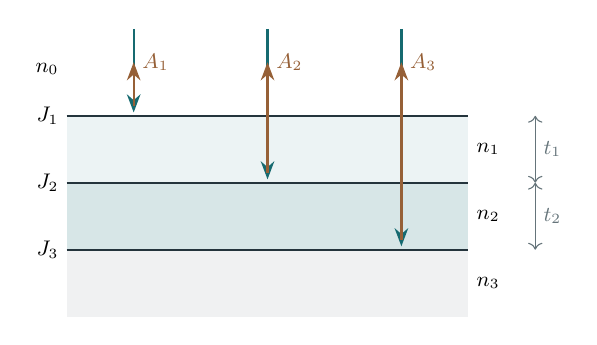
\begin{tikzpicture}[scale=.85,transform shape]

\fill[accent!8] (-3,1) rectangle (3,2);
\fill[accent!17] (-3,0) rectangle (3,1);
\fill[muted!10] (-3,-1) rectangle (3,0);
\foreach \y/\p in {2/J_1,1/J_2,0/J_3}{\draw[object] (-3,\y)--(3,\y);\node[left] at (-3,\y) {$\p$};}
\node[left] at (-3,2.7) {$n_0$};
\node[right] at (3,1.5) {$n_1$};\node[right] at (3,.5) {$n_2$};
\node[right] at (3,-.5) {$n_3$};
\draw[axis,<->] (4,1)--(4,2) node[midway,right] {$t_1$};
\draw[axis,<->] (4,0)--(4,1) node[midway,right] {$t_2$};
\draw[motion] (-2,3.3)--(-2,2.05);
\draw[motion] (0,3.3)--(0,1.05);
\draw[motion] (2,3.3)--(2,.05);
\draw[force] (-2,2.15)--(-2,2.8) node[right] {$A_1$};
\draw[force] (0,1.15)--(0,2.8) node[right] {$A_2$};
\draw[force] (2,.15)--(2,2.8) node[right] {$A_3$};

\end{tikzpicture}
\figcaption{图光试.5\quad 三条法向反射路径分列表示，$n_0<n_1<n_2,\ n_2>n_3$。}
\end{minipage}\end{center}

\Needspace{6\baselineskip}\subsection*{解答}


图光试.5的三个界面分别记为$J_1,J_2,J_3$。从低折射率入射到高折射率的反射振幅变号，相位增加$\pi$；从高到低反射不增加该相位。因此三次反射附加相位依次为
\[
\pi,\qquad \pi,\qquad 0.
\]
\begin{center}\begin{minipage}{.98\linewidth}\centering
\begin{tikzpicture}[scale=.7,transform shape]

\fill[accent!8] (-3,1) rectangle (3,2);
\fill[accent!17] (-3,0) rectangle (3,1);
\fill[muted!10] (-3,-1) rectangle (3,0);
\foreach \y/\p in {2/J_1,1/J_2,0/J_3}{\draw[object] (-3,\y)--(3,\y);\node[left] at (-3,\y) {$\p$};}
\node[left] at (-3,2.7) {$n_0$};
\node[right] at (3,1.5) {$n_1$};\node[right] at (3,.5) {$n_2$};
\node[right] at (3,-.5) {$n_3$};
\draw[axis,<->] (4,1)--(4,2) node[midway,right] {$t_1$};
\draw[axis,<->] (4,0)--(4,1) node[midway,right] {$t_2$};
\draw[motion] (-2,3.3)--(-2,2.05);
\draw[motion] (0,3.3)--(0,1.05);
\draw[motion] (2,3.3)--(2,.05);
\draw[force] (-2,2.15)--(-2,2.8) node[right] {$A_1$};
\draw[force] (0,1.15)--(0,2.8) node[right] {$A_2$};
\draw[force] (2,.15)--(2,2.8) node[right] {$A_3$};

\node[align=left] at (8,2) {$J_1:\ \pi$\\$J_2:\ \pi$\\$J_3:\ 0$};
\node[align=left] at (8,0) {第二束往返：$2n_1t_1$\\第三束往返：$2n_1t_1+2n_2t_2$};

\end{tikzpicture}
\figcaption{解图光试.5A\quad 三界面的反射相变与两层往返传播相位分别计入，第三束带相对负号。}
\end{minipage}\end{center}
解图光试.5A把第二、三束在膜内的往返路程分别标为$2n_1t_1$与$2n_1t_1+2n_2t_2$。令
\[
\delta_1=\frac{4\pi n_1t_1}{\lambda},\qquad
\delta_2=\frac{4\pi n_2t_2}{\lambda}.
\]
去掉公共的第一束相位，并取三束共同振幅为$A>0$，复振幅可写成
\[
\widetilde A_1=A,\qquad
\widetilde A_2=Ae^{\mathrm j\delta_1},\qquad
\widetilde A_3=-Ae^{\mathrm j(\delta_1+\delta_2)}.
\]
第三束前的负号保留了它与前两束反射相位相差$\pi$这一事实。要求总强度为零，就是
\[
1+e^{\mathrm j\delta_1}
-e^{\mathrm j(\delta_1+\delta_2)}=0.
\]
\begin{center}\begin{minipage}{.98\linewidth}\centering
\begin{tikzpicture}[scale=.8,transform shape]

\draw[motion] (0,0)--(2,0) node[right] {$A_1$};
\draw[motion] (0,0)--(-1,1.732) node[above] {$A_2$};
\draw[motion] (0,0)--(-1,-1.732) node[below] {$A_3$};
\draw[guide] (0,0) circle (2);
\node at (0,3) {共同起点：相位相隔$120^\circ$};
\begin{scope}[xshift=6cm]
\draw[motion] (0,0)--(2,0) node[midway,below] {$A_1$};
\draw[motion] (2,0)--(1,1.732) node[midway,right] {$A_2$};
\draw[motion] (1,1.732)--(0,0) node[midway,left] {$A_3$};
\node at (1,3) {首尾闭合：合振幅为零};
\end{scope}
\node at (3,-3) {$\delta_1=2\pi/3,\quad\delta_2=5\pi/3$时的三相量};

\end{tikzpicture}
\figcaption{解图光试.5B\quad 方向角与矢量首尾相加是同一零和条件的两种画法。}
\end{minipage}\end{center}
解图光试.5B中三条等长相量在零和时首尾组成等边三角形，等价于从共同起点画出时方向依次相差$120^\circ$。对零和方程取模，可具体求得：
\[
|1+e^{\mathrm j\delta_1}|^2=1
\quad\Longrightarrow\quad
2+2\cos\delta_1=1.
\]
所以$\cos\delta_1=-1/2$，在模$2\pi$意义下只有
\[
\delta_1\equiv\frac{2\pi}{3}\quad\text{或}\quad
\delta_1\equiv\frac{4\pi}{3}.
\]
对第一支$\delta_1=2\pi/3$，$1+e^{2\pi\mathrm j/3}=e^{\pi\mathrm j/3}$，故$\delta_1+\delta_2\equiv\pi/3$，得到$\delta_2\equiv5\pi/3$。对第二支$\delta_1=4\pi/3$，和为$e^{-\pi\mathrm j/3}$，所以$\delta_2\equiv\pi/3$。每一层增加$\lambda/(2n)$只使相应传播相位增加$2\pi$。分别加上独立的整周期后，得到两族正厚度解：
\[
\begin{array}{c|c|c}
&t_1&t_2\\ \hline
\text{第一族}&\displaystyle\frac{\lambda}{6n_1}
+m\frac{\lambda}{2n_1}
&\displaystyle\frac{5\lambda}{12n_2}
+p\frac{\lambda}{2n_2}\\[2mm]
\text{第二族}&\displaystyle\frac{\lambda}{3n_1}
+m\frac{\lambda}{2n_1}
&\displaystyle\frac{\lambda}{12n_2}
+p\frac{\lambda}{2n_2}
\end{array}
\qquad m,p=0,1,2,\ldots.
\]
例如第一族的最小相位为$\delta_1=2\pi/3$、$\delta_2=5\pi/3$，第三束相对于第一束的总相位为
$\delta_1+\delta_2+\pi\equiv4\pi/3$，三束相位正是$0,2\pi/3,4\pi/3$。

按题意先最小化$t_1$，第一族给出的$\lambda/(6n_1)$小于第二族的$\lambda/(3n_1)$；再在第一族内取$p=0$，故
\[
\boxed{t_{1,\min}=\frac{\lambda}{6n_1},\qquad
t_{2,\min\,|\,t_{1,\min}}=\frac{5\lambda}{12n_2}}.
\]
单独追求$t_2$最小则应选第二族，$t_2=\lambda/(12n_2)$，同时$t_1=\lambda/(3n_1)$。两层的厚度由同一支相位条件配对。若比较两组总厚度，第二族的最小总厚度减去第一族的最小总厚度为
\[
\left(\frac{\lambda}{3n_1}+\frac{\lambda}{12n_2}\right)
-\left(\frac{\lambda}{6n_1}+\frac{5\lambda}{12n_2}\right)
=\frac{\lambda(n_2-2n_1)}{6n_1n_2}.
\]
所以 $n_2<2n_1$ 时，先使 $t_2$ 最小所得组合的总厚度也较小；$n_2=2n_1$ 时总厚度相同；$n_2>2n_1$ 时，先使 $t_1$ 最小所得组合的总厚度较小。

题设将三个一次反射分量的共同幅度规定为$A$。若考虑其余多次往返或改变三个幅度，便以对应传播和反射系数构成全部复振幅之和；膜厚扰动时，各层传播相位按$4\pi n_jt_j/\lambda$随厚度改变。
还可把第一族写成直观的光程式：$2n_1t_1=\lambda/3$，而第一、第三束的反射相位相差$\pi$，故$2n_1t_1+2n_2t_2=7\lambda/6$；相减得到$2n_2t_2=5\lambda/6$。解图光试.5C按这两个往返光程画出相位逐段累积。
\begin{center}\begin{minipage}{.98\linewidth}\centering
\begin{tikzpicture}[scale=0.72,transform shape]
\draw[axis] (0,0)--(6.2,0);\draw[axis] (0,0)--(0,3.4000000000000004);
\draw[thin,color=muted] (0.0000000,0)--(0.0000000,-.07);\node[below] at (0.0000000,-.09) {参考};
\draw[thin,color=muted] (2.0000000,0)--(2.0000000,-.07);\node[below] at (2.0000000,-.09) {第一层往返};
\draw[thin,color=muted] (4.0000000,0)--(4.0000000,-.07);\node[below] at (4.0000000,-.09) {第二层往返};
\draw[thin,color=muted] (6.0000000,0)--(6.0000000,-.07);\node[below] at (6.0000000,-.09) {相对反射};
\draw[thin,color=muted] (0,0.0000000)--(-.07,0.0000000);\node[left] at (-.09,0.0000000) {$0$};
\draw[thin,color=muted] (0,0.5925926)--(-.07,0.5925926);\node[left] at (-.09,0.5925926) {$2/3$};
\draw[thin,color=muted] (0,2.0740741)--(-.07,2.0740741);\node[left] at (-.09,2.0740741) {$7/3$};
\draw[thin,color=muted] (0,2.9629630)--(-.07,2.9629630);\node[left] at (-.09,2.9629630) {$10/3$};
\node[below] at (3.0,-.64) {逐段累计};\node[above right] at (0,3.45) {相位除以$\pi$};
\draw[traj] plot coordinates {(0.0000000,0.0000000) (2.0000000,0.5925926) (4.0000000,2.0740741) (6.0000000,2.9629630)};
\draw[traj] (.1,-1.05)--(.7,-1.05);\node[right] at (.85,-1.05) {第三束传播与相对反射相位};\end{tikzpicture}
\figcaption{解图光试.5C\quad 传播相位之和为 $7\pi/3$，再计相对反射 $\pi$ 后等效方向为 $4\pi/3$}
\end{minipage}\end{center}


\Needspace{13\baselineskip}

\pdfbookmark[2]{第 6 题 棱镜色散与衍射限制的分辨本领}{q6}

\section*{第 6 题\quad 棱镜色散与衍射限制的分辨本领}\label{q:6}


棱镜光谱仪中的等腰三棱镜$ABC$顶角为$\beta$，底边$BC=L$，两腰长为$b$，材料折射率为$n(\lambda)$。中心波长$\lambda$的光在最小偏向角条件下通过棱镜，入射面$AB$被均匀、充分照明。

把有限入射面视为宽度$b$的单缝，考虑它对出射主峰的衍射展宽，按瑞利判据推导分辨本领$\mathcal R=\lambda/\delta\lambda$。保留入射、折射角和有效投影孔径的关系，说明色散率符号如何处理。

采用窄谱带一阶近似和夫琅禾费衍射模型，忽略狭缝宽度、像差及探测器像素造成的其他展宽。


\begin{center}\begin{minipage}{.98\linewidth}\centering
\begin{tikzpicture}[scale=.8,transform shape]

\coordinate (A) at (0,3);\coordinate (B) at (-2,0);\coordinate (C) at (2,0);
\fill[accent!8] (A)--(B)--(C)--cycle;\draw[object] (A)--(B)--(C)--cycle;
\node[above] at (A) {$A$};\node[below left] at (B) {$B$};\node[below right] at (C) {$C$};
\node at (0,2.25) {$\beta$};
\node[left] at (-1.3,1.7) {$b$};\node[right] at (1.3,1.7) {$b$};
\draw[axis,<->] (-2,-.8)--(2,-.8) node[midway,below] {$L$};

\draw[motion] (-4,.565)--(-1,1.5)--(1,1.5)--(4,.565);
\node at (0,4) {等腰棱镜，中心波长按最小偏向通过};

\end{tikzpicture}
\figcaption{图光试.6\quad 满照面宽与底边长度不同，中心光路关于顶角平分线对称。}
\end{minipage}\end{center}

\Needspace{6\baselineskip}\subsection*{解答}


图光试.6中$\beta$为顶角，$BC=L$，$AB=AC=b$。最小偏向时光路关于顶角平分线对称，入射角与出射角均为$i$，内部两折射角均为$r=\beta/2$。由折射定律
\[
\sin i=n\sin\frac\beta2,\qquad
\delta_{\min}=2i-\beta.
\]
因此
\[
n=\frac{\sin[(\beta+\delta_{\min})/2]}{\sin(\beta/2)},
\qquad
\boxed{\frac{d\delta_{\min}}{dn}
=\frac{2\sin(\beta/2)}{\cos i}}.
\]
\begin{center}\begin{minipage}{.98\linewidth}\centering
\begin{tikzpicture}[scale=.75,transform shape]

\coordinate (A) at (0,3);\coordinate (B) at (-2,0);\coordinate (C) at (2,0);
\fill[accent!8] (A)--(B)--(C)--cycle;\draw[object] (A)--(B)--(C)--cycle;
\node[above] at (A) {$A$};\node[below left] at (B) {$B$};\node[below right] at (C) {$C$};
\node at (0,2.25) {$\beta$};
\node[left] at (-1.3,2.7) {$b$};\node[right] at (1.3,1.7) {$b$};
\draw[axis,<->] (-2,-.8)--(2,-.8) node[midway,below] {$L$};

\draw[guide] (-5.54,1.274)--(0,3);
\draw[guide] (-4.864,-.893)--(-2,0);
\draw[axis,<->] (-4.864,-.893)--(-5.54,1.274) node[midway,left] {$w$};
\draw[motion] (-4,.565)--(-1,1.5)--(1,1.5)--(4,.565);
\draw[guide] (-2,2.167)--(0,.833);
\draw[guide] (0,.833)--(2,2.167);
\draw[guide] (-4,1.5)--(4,1.5);
\draw[object] (-1,1.5)++(146.31:.65) arc[start angle=146.31,end angle=197.31,radius=.65];
\node at (-1.8,1.62) {$i$};
\draw[object] (-1,1.5)++(-33.69:.6) arc[start angle=-33.69,end angle=0,radius=.6];
\node at (-.25,1.25) {$r$};
\node[align=left] at (6,2.3) {$r=\beta/2$\\$\sin i=n\sin(\beta/2)$\\$w=b\cos i$};
\node[align=left] at (6,.2) {法线用虚线表示\\$i$从法线量\\$w$垂直光束};

\end{tikzpicture}
\figcaption{解图光试.6A\quad 最小偏向时入、出射角相同，面宽投影给有效孔径。}
\end{minipage}\end{center}
解图光试.6A中，入射面宽$b$对垂直光束截面的投影为
\[
w=b\cos i.
\]
$w$ 是用来计算横向衍射相位的有效孔径。在最小偏向时，两侧的入射面和出射面对称，出射截面的有效孔径也为 $w$。这里取 $n\sin(\beta/2)<1$，使折射光出射而且 $\cos i>0$。单缝主峰中心到第一暗纹的半角宽为
\[
\boxed{\Delta\theta_{\rm dif}\simeq\frac{\lambda}{w}
=\frac{\lambda}{b\cos i}}.
\]
也可从孔径上的相位积分看到：偏离主方向$\theta$时，振幅正比于
$\int_{-w/2}^{w/2}e^{\mathrm jkx\sin\theta}dx$，积分等于$2\sin(kw\sin\theta/2)/(k\sin\theta)$，归一化强度为$[\sin u/u]^2$，$u=\pi w\sin\theta/\lambda$。其第一次为零满足
$w\sin\theta=\lambda$。当 $w\gg\lambda$ 时，首暗纹位于近轴小角范围。瑞利角间距取单峰中心到一侧首暗纹的角距；图 B 据此把一条线的中心放在另一条线的首零点。
\begin{center}\begin{minipage}{.98\linewidth}\centering
\begin{tikzpicture}[scale=.9,transform shape]

\draw[axis] (-2.5,0)--(3.6,0) node[right] {$\theta/(\lambda/w)$};
\draw[axis] (-2.3,0)--(-2.3,4.8) node[above] {相对强度};
\draw[traj,domain=-2:3,samples=350] plot (\x,{4*pow(sin(180*(\x+.00001))/(pi*(\x+.00001)),2)});
\draw[force,domain=-2:3,samples=350] plot (\x,{4*pow(sin(180*(\x-1+.00001))/(pi*(\x-1+.00001)),2)});
\draw[guide] (0,0)--(0,4.3);\draw[guide] (1,0)--(1,4.3);
\node[below] at (0,0) {$0$};\node[below] at (1,0) {$1$};
\draw[axis,<->] (0,4.6)--(1,4.6);
\node[align=left] at (6,2.8) {一个峰中心落在\\另一峰的第一暗纹\\$\Delta\theta=\lambda/w$};
\node at (2,-1.2) {$\left|d\delta/d\lambda\right|\delta\lambda=\lambda/(b\cos i)$};

\end{tikzpicture}
\figcaption{解图光试.6B\quad 瑞利判据比较中心间距与单峰半角宽，色散方向取绝对值。}
\end{minipage}\end{center}
解图光试.6B按瑞利判据把一条谱线的主峰放在另一条的第一暗纹处。相邻波长的方向间隔，在一阶近似下为
\[
\Delta\theta_{\rm disp}
=\left|\frac{d\delta_{\min}}{d\lambda}\right|\delta\lambda
=\frac{2\sin(\beta/2)}{\cos i}
\left|\frac{dn}{d\lambda}\right|\delta\lambda.
\]
令它等于衍射半角宽，
\[
\frac{2\sin(\beta/2)}{\cos i}
\left|\frac{dn}{d\lambda}\right|\delta\lambda
=\frac{\lambda}{b\cos i}.
\]
两侧的$\cos i$抵消，得到
\[
\mathcal R=\frac{\lambda}{\delta\lambda}
=2b\sin\frac\beta2\left|\frac{dn}{d\lambda}\right|.
\]
等腰三角形几何关系$L=2b\sin(\beta/2)$给出
\[
\boxed{\mathcal R=L\left|\frac{dn}{d\lambda}\right|}.
\]
普通正常色散常有$dn/d\lambda<0$，分辨本领则是正数，故取导数的绝对值。$L$与$d n/d\lambda$的长度单位应一致，结果无量纲。

相邻波长实际通过同一个固定棱镜。为说明其角色散与上式的一阶联系，在固定入射角下微分两次折射关系。令入射角为$i$，写
\[
\sin i=n\sin r_1,\quad r_2=\beta-r_1,\quad
\sin e=n\sin r_2.
\]
固定$i$微分第一式得到$0=\sin r_1+n\cos r_1\,dr_1/dn$，即$dr_1/dn=-\tan r_1/n$。由$r_1+r_2=\beta$，$dr_2/dn=\tan r_1/n$；再对出射式求导，有$\cos e\,de/dn=\sin r_2+n\cos r_2\,dr_2/dn$，继而
\[
\frac{de}{dn}
=\frac{\sin r_2+\cos r_2\tan r_1}{\cos e}
=\frac{\sin\beta}{\cos r_1\cos e}.
\]
在中心波长的最小偏向点$r_1=r_2=\beta/2,e=i$，这正好等于
$2\sin(\beta/2)/\cos i$，所以一阶色散计算适用于固定棱镜的窄谱带。

若入射面只被部分照明，应把$b$换成实际受照宽度$b_{\rm eff}$，结果中的$L$相应换为$2b_{\rm eff}\sin(\beta/2)$。此值对应充分照明和仅含孔径衍射的条件；实际狭缝宽度、像差与探测器响应可继续参与总谱线展宽。
解图光试.6C将角色散的两条窄谱线同时画在投影孔径的归一化角坐标$q=w\theta/\lambda$上；在瑞利距离下两中心相差1，某一条的中心与另一条的首零点重合。若两条谱线彼此不相干，探测强度是两个单峰强度相加，图中的总曲线保留两个中心间的凹陷。
\begin{center}\begin{minipage}{.98\linewidth}\centering
\begin{tikzpicture}[scale=0.72,transform shape]
\draw[axis] (0,0)--(6.2,0);\draw[axis] (0,0)--(0,3.4000000000000004);
\draw[thin,color=muted] (0.6000000,0)--(0.6000000,-.07);\node[below] at (0.6000000,-.09) {$-2$};
\draw[thin,color=muted] (2.4000000,0)--(2.4000000,-.07);\node[below] at (2.4000000,-.09) {$-1/2$};
\draw[thin,color=muted] (3.6000000,0)--(3.6000000,-.07);\node[below] at (3.6000000,-.09) {$1/2$};
\draw[thin,color=muted] (5.4000000,0)--(5.4000000,-.07);\node[below] at (5.4000000,-.09) {$2$};
\draw[thin,color=muted] (0,0.0000000)--(-.07,0.0000000);\node[left] at (-.09,0.0000000) {$0$};
\draw[thin,color=muted] (0,1.4545455)--(-.07,1.4545455);\node[left] at (-.09,1.4545455) {$.5$};
\draw[thin,color=muted] (0,2.9090909)--(-.07,2.9090909);\node[left] at (-.09,2.9090909) {$1$};
\node[below] at (3.0,-.64) {$q=w\theta/\lambda$};\node[above right] at (0,3.45) {归一化强度};
\draw[traj] plot coordinates {(0.0000000,0.0000000) (0.0120000,0.0000734) (0.0240000,0.0002964) (0.0360000,0.0006726) (0.0480000,0.0012053) (0.0600000,0.0018969) (0.0720000,0.0027498) (0.0840000,0.0037655) (0.0960000,0.0049451) (0.1080000,0.0062889) (0.1200000,0.0077968) (0.1320000,0.0094681) (0.1440000,0.0113014) (0.1560000,0.0132947) (0.1680000,0.0154455) (0.1800000,0.0177504) (0.1920000,0.0202056) (0.2040000,0.0228067) (0.2160000,0.0255484) (0.2280000,0.0284251) (0.2400000,0.0314304) (0.2520000,0.0345574) (0.2640000,0.0377985) (0.2760000,0.0411456) (0.2880000,0.0445901) (0.3000000,0.0481229) (0.3120000,0.0517341) (0.3240000,0.0554136) (0.3360000,0.0591508) (0.3480000,0.0629347) (0.3600000,0.0667536) (0.3720000,0.0705959) (0.3840000,0.0744494) (0.3960000,0.0783016) (0.4080000,0.0821398) (0.4200000,0.0859511) (0.4320000,0.0897224) (0.4440000,0.0934406) (0.4560000,0.0970923) (0.4680000,0.1006642) (0.4800000,0.1041430) (0.4920000,0.1075156) (0.5040000,0.1107687) (0.5160000,0.1138895) (0.5280000,0.1168652) (0.5400000,0.1196834) (0.5520000,0.1223319) (0.5640000,0.1247990) (0.5760000,0.1270734) (0.5880000,0.1291442) (0.6000000,0.1310011) (0.6120000,0.1326344) (0.6240000,0.1340351) (0.6360000,0.1351946) (0.6480000,0.1361055) (0.6600000,0.1367607) (0.6720000,0.1371543) (0.6840000,0.1372812) (0.6960000,0.1371370) (0.7080000,0.1367186) (0.7200000,0.1360236) (0.7320000,0.1350508) (0.7440000,0.1338001) (0.7560000,0.1322725) (0.7680000,0.1304701) (0.7800000,0.1283961) (0.7920000,0.1260550) (0.8040000,0.1234526) (0.8160000,0.1205957) (0.8280000,0.1174926) (0.8400000,0.1141527) (0.8520000,0.1105867) (0.8640000,0.1068065) (0.8760000,0.1028256) (0.8880000,0.0986584) (0.9000000,0.0943208) (0.9120000,0.0898299) (0.9240000,0.0852040) (0.9360000,0.0804627) (0.9480000,0.0756269) (0.9600000,0.0707184) (0.9720000,0.0657605) (0.9840000,0.0607774) (0.9960000,0.0557946) (1.0080000,0.0508384) (1.0200000,0.0459362) (1.0320000,0.0411166) (1.0440000,0.0364087) (1.0560000,0.0318428) (1.0680000,0.0274498) (1.0800000,0.0232615) (1.0920000,0.0193101) (1.1040000,0.0156288) (1.1160000,0.0122511) (1.1280000,0.0092108) (1.1400000,0.0065425) (1.1520000,0.0042808) (1.1640000,0.0024606) (1.1760000,0.0011170) (1.1880000,0.0002851) (1.2000000,0.0000000) (1.2120000,0.0002967) (1.2240000,0.0012100) (1.2360000,0.0027744) (1.2480000,0.0050240) (1.2600000,0.0079924) (1.2720000,0.0117126) (1.2840000,0.0162172) (1.2960000,0.0215376) (1.3080000,0.0277048) (1.3200000,0.0347486) (1.3320000,0.0426978) (1.3440000,0.0515801) (1.3560000,0.0614219) (1.3680000,0.0722486) (1.3800000,0.0840840) (1.3920000,0.0969503) (1.4040000,0.1108684) (1.4160000,0.1258574) (1.4280000,0.1419348) (1.4400000,0.1591164) (1.4520000,0.1774159) (1.4640000,0.1968453) (1.4760000,0.2174146) (1.4880000,0.2391316) (1.5000000,0.2620023) (1.5120000,0.2860301) (1.5240000,0.3112168) (1.5360000,0.3375614) (1.5480000,0.3650610) (1.5600000,0.3937103) (1.5720000,0.4235016) (1.5840000,0.4544248) (1.5960000,0.4864676) (1.6080000,0.5196153) (1.6200000,0.5538506) (1.6320000,0.5891539) (1.6440000,0.6255033) (1.6560000,0.6628745) (1.6680000,0.7012406) (1.6800000,0.7405727) (1.6920000,0.7808393) (1.7040000,0.8220068) (1.7160000,0.8640391) (1.7280000,0.9068981) (1.7400000,0.9505436) (1.7520000,0.9949329) (1.7640000,1.0400217) (1.7760000,1.0857634) (1.7880000,1.1321097) (1.8000000,1.1790101) (1.8120000,1.2264128) (1.8240000,1.2742640) (1.8360000,1.3225084) (1.8480000,1.3710890) (1.8600000,1.4199478) (1.8720000,1.4690251) (1.8840000,1.5182601) (1.8960000,1.5675911) (1.9080000,1.6169552) (1.9200000,1.6662886) (1.9320000,1.7155268) (1.9440000,1.7646049) (1.9560000,1.8134570) (1.9680000,1.8620172) (1.9800000,1.9102193) (1.9920000,1.9579967) (2.0040000,2.0052831) (2.0160000,2.0520120) (2.0280000,2.0981175) (2.0400000,2.1435338) (2.0520000,2.1881957) (2.0640000,2.2320386) (2.0760000,2.2749988) (2.0880000,2.3170133) (2.1000000,2.3580203) (2.1120000,2.3979589) (2.1240000,2.4367698) (2.1360000,2.4743948) (2.1480000,2.5107773) (2.1600000,2.5458624) (2.1720000,2.5795968) (2.1840000,2.6119292) (2.1960000,2.6428100) (2.2080000,2.6721920) (2.2200000,2.7000298) (2.2320000,2.7262806) (2.2440000,2.7509035) (2.2560000,2.7738606) (2.2680000,2.7951158) (2.2800000,2.8146362) (2.2920000,2.8323913) (2.3040000,2.8483531) (2.3160000,2.8624967) (2.3280000,2.8747998) (2.3400000,2.8852432) (2.3520000,2.8938103) (2.3640000,2.9004876) (2.3760000,2.9052647) (2.3880000,2.9081340) (2.4000000,2.9090909) (2.4120000,2.9081340) (2.4240000,2.9052647) (2.4360000,2.9004876) (2.4480000,2.8938103) (2.4600000,2.8852432) (2.4720000,2.8747998) (2.4840000,2.8624967) (2.4960000,2.8483531) (2.5080000,2.8323913) (2.5200000,2.8146362) (2.5320000,2.7951158) (2.5440000,2.7738606) (2.5560000,2.7509035) (2.5680000,2.7262806) (2.5800000,2.7000298) (2.5920000,2.6721920) (2.6040000,2.6428100) (2.6160000,2.6119292) (2.6280000,2.5795968) (2.6400000,2.5458624) (2.6520000,2.5107773) (2.6640000,2.4743948) (2.6760000,2.4367698) (2.6880000,2.3979589) (2.7000000,2.3580203) (2.7120000,2.3170133) (2.7240000,2.2749988) (2.7360000,2.2320386) (2.7480000,2.1881957) (2.7600000,2.1435338) (2.7720000,2.0981175) (2.7840000,2.0520120) (2.7960000,2.0052831) (2.8080000,1.9579967) (2.8200000,1.9102193) (2.8320000,1.8620172) (2.8440000,1.8134570) (2.8560000,1.7646049) (2.8680000,1.7155268) (2.8800000,1.6662886) (2.8920000,1.6169552) (2.9040000,1.5675911) (2.9160000,1.5182601) (2.9280000,1.4690251) (2.9400000,1.4199478) (2.9520000,1.3710890) (2.9640000,1.3225084) (2.9760000,1.2742640) (2.9880000,1.2264128) (3.0000000,1.1790101) (3.0120000,1.1321097) (3.0240000,1.0857634) (3.0360000,1.0400217) (3.0480000,0.9949329) (3.0600000,0.9505436) (3.0720000,0.9068981) (3.0840000,0.8640391) (3.0960000,0.8220068) (3.1080000,0.7808393) (3.1200000,0.7405727) (3.1320000,0.7012406) (3.1440000,0.6628745) (3.1560000,0.6255033) (3.1680000,0.5891539) (3.1800000,0.5538506) (3.1920000,0.5196153) (3.2040000,0.4864676) (3.2160000,0.4544248) (3.2280000,0.4235016) (3.2400000,0.3937103) (3.2520000,0.3650610) (3.2640000,0.3375614) (3.2760000,0.3112168) (3.2880000,0.2860301) (3.3000000,0.2620023) (3.3120000,0.2391316) (3.3240000,0.2174146) (3.3360000,0.1968453) (3.3480000,0.1774159) (3.3600000,0.1591164) (3.3720000,0.1419348) (3.3840000,0.1258574) (3.3960000,0.1108684) (3.4080000,0.0969503) (3.4200000,0.0840840) (3.4320000,0.0722486) (3.4440000,0.0614219) (3.4560000,0.0515801) (3.4680000,0.0426978) (3.4800000,0.0347486) (3.4920000,0.0277048) (3.5040000,0.0215376) (3.5160000,0.0162172) (3.5280000,0.0117126) (3.5400000,0.0079924) (3.5520000,0.0050240) (3.5640000,0.0027744) (3.5760000,0.0012100) (3.5880000,0.0002967) (3.6000000,0.0000000) (3.6120000,0.0002851) (3.6240000,0.0011170) (3.6360000,0.0024606) (3.6480000,0.0042808) (3.6600000,0.0065425) (3.6720000,0.0092108) (3.6840000,0.0122511) (3.6960000,0.0156288) (3.7080000,0.0193101) (3.7200000,0.0232615) (3.7320000,0.0274498) (3.7440000,0.0318428) (3.7560000,0.0364087) (3.7680000,0.0411166) (3.7800000,0.0459362) (3.7920000,0.0508384) (3.8040000,0.0557946) (3.8160000,0.0607774) (3.8280000,0.0657605) (3.8400000,0.0707184) (3.8520000,0.0756269) (3.8640000,0.0804627) (3.8760000,0.0852040) (3.8880000,0.0898299) (3.9000000,0.0943208) (3.9120000,0.0986584) (3.9240000,0.1028256) (3.9360000,0.1068065) (3.9480000,0.1105867) (3.9600000,0.1141527) (3.9720000,0.1174926) (3.9840000,0.1205957) (3.9960000,0.1234526) (4.0080000,0.1260550) (4.0200000,0.1283961) (4.0320000,0.1304701) (4.0440000,0.1322725) (4.0560000,0.1338001) (4.0680000,0.1350508) (4.0800000,0.1360236) (4.0920000,0.1367186) (4.1040000,0.1371370) (4.1160000,0.1372812) (4.1280000,0.1371543) (4.1400000,0.1367607) (4.1520000,0.1361055) (4.1640000,0.1351946) (4.1760000,0.1340351) (4.1880000,0.1326344) (4.2000000,0.1310011) (4.2120000,0.1291442) (4.2240000,0.1270734) (4.2360000,0.1247990) (4.2480000,0.1223319) (4.2600000,0.1196834) (4.2720000,0.1168652) (4.2840000,0.1138895) (4.2960000,0.1107687) (4.3080000,0.1075156) (4.3200000,0.1041430) (4.3320000,0.1006642) (4.3440000,0.0970923) (4.3560000,0.0934406) (4.3680000,0.0897224) (4.3800000,0.0859511) (4.3920000,0.0821398) (4.4040000,0.0783016) (4.4160000,0.0744494) (4.4280000,0.0705959) (4.4400000,0.0667536) (4.4520000,0.0629347) (4.4640000,0.0591508) (4.4760000,0.0554136) (4.4880000,0.0517341) (4.5000000,0.0481229) (4.5120000,0.0445901) (4.5240000,0.0411456) (4.5360000,0.0377985) (4.5480000,0.0345574) (4.5600000,0.0314304) (4.5720000,0.0284251) (4.5840000,0.0255484) (4.5960000,0.0228067) (4.6080000,0.0202056) (4.6200000,0.0177504) (4.6320000,0.0154455) (4.6440000,0.0132947) (4.6560000,0.0113014) (4.6680000,0.0094681) (4.6800000,0.0077968) (4.6920000,0.0062889) (4.7040000,0.0049451) (4.7160000,0.0037655) (4.7280000,0.0027498) (4.7400000,0.0018969) (4.7520000,0.0012053) (4.7640000,0.0006726) (4.7760000,0.0002964) (4.7880000,0.0000734) (4.8000000,0.0000000) (4.8120000,0.0000720) (4.8240000,0.0002848) (4.8360000,0.0006335) (4.8480000,0.0011126) (4.8600000,0.0017164) (4.8720000,0.0024388) (4.8840000,0.0032734) (4.8960000,0.0042135) (4.9080000,0.0052523) (4.9200000,0.0063824) (4.9320000,0.0075966) (4.9440000,0.0088874) (4.9560000,0.0102471) (4.9680000,0.0116681) (4.9800000,0.0131424) (4.9920000,0.0146622) (5.0040000,0.0162198) (5.0160000,0.0178071) (5.0280000,0.0194165) (5.0400000,0.0210402) (5.0520000,0.0226706) (5.0640000,0.0243001) (5.0760000,0.0259215) (5.0880000,0.0275276) (5.1000000,0.0291114) (5.1120000,0.0306661) (5.1240000,0.0321853) (5.1360000,0.0336626) (5.1480000,0.0350922) (5.1600000,0.0364684) (5.1720000,0.0377859) (5.1840000,0.0390395) (5.1960000,0.0402246) (5.2080000,0.0413369) (5.2200000,0.0423725) (5.2320000,0.0433276) (5.2440000,0.0441992) (5.2560000,0.0449843) (5.2680000,0.0456805) (5.2800000,0.0462858) (5.2920000,0.0467985) (5.3040000,0.0472172) (5.3160000,0.0475412) (5.3280000,0.0477700) (5.3400000,0.0479033) (5.3520000,0.0479414) (5.3640000,0.0478851) (5.3760000,0.0477352) (5.3880000,0.0474931) (5.4000000,0.0471604) (5.4120000,0.0467392) (5.4240000,0.0462318) (5.4360000,0.0456408) (5.4480000,0.0449691) (5.4600000,0.0442198) (5.4720000,0.0433965) (5.4840000,0.0425027) (5.4960000,0.0415424) (5.5080000,0.0405197) (5.5200000,0.0394388) (5.5320000,0.0383041) (5.5440000,0.0371204) (5.5560000,0.0358921) (5.5680000,0.0346243) (5.5800000,0.0333217) (5.5920000,0.0319894) (5.6040000,0.0306324) (5.6160000,0.0292557) (5.6280000,0.0278643) (5.6400000,0.0264634) (5.6520000,0.0250578) (5.6640000,0.0236527) (5.6760000,0.0222527) (5.6880000,0.0208629) (5.7000000,0.0194878) (5.7120000,0.0181320) (5.7240000,0.0168001) (5.7360000,0.0154962) (5.7480000,0.0142245) (5.7600000,0.0129891) (5.7720000,0.0117936) (5.7840000,0.0106416) (5.7960000,0.0095365) (5.8080000,0.0084815) (5.8200000,0.0074793) (5.8320000,0.0065327) (5.8440000,0.0056441) (5.8560000,0.0048157) (5.8680000,0.0040494) (5.8800000,0.0033468) (5.8920000,0.0027093) (5.9040000,0.0021380) (5.9160000,0.0016338) (5.9280000,0.0011973) (5.9400000,0.0008289) (5.9520000,0.0005285) (5.9640000,0.0002959) (5.9760000,0.0001309) (5.9880000,0.0000325) (6.0000000,0.0000000)};
\draw[traj] (.1,-1.05)--(.7,-1.05);\node[right] at (.85,-1.05) {左谱线};\draw[dashed,thick,color=warm] plot coordinates {(0.0000000,0.0000000) (0.0120000,0.0000325) (0.0240000,0.0001309) (0.0360000,0.0002959) (0.0480000,0.0005285) (0.0600000,0.0008289) (0.0720000,0.0011973) (0.0840000,0.0016338) (0.0960000,0.0021380) (0.1080000,0.0027093) (0.1200000,0.0033468) (0.1320000,0.0040494) (0.1440000,0.0048157) (0.1560000,0.0056441) (0.1680000,0.0065327) (0.1800000,0.0074793) (0.1920000,0.0084815) (0.2040000,0.0095365) (0.2160000,0.0106416) (0.2280000,0.0117936) (0.2400000,0.0129891) (0.2520000,0.0142245) (0.2640000,0.0154962) (0.2760000,0.0168001) (0.2880000,0.0181320) (0.3000000,0.0194878) (0.3120000,0.0208629) (0.3240000,0.0222527) (0.3360000,0.0236527) (0.3480000,0.0250578) (0.3600000,0.0264634) (0.3720000,0.0278643) (0.3840000,0.0292557) (0.3960000,0.0306324) (0.4080000,0.0319894) (0.4200000,0.0333217) (0.4320000,0.0346243) (0.4440000,0.0358921) (0.4560000,0.0371204) (0.4680000,0.0383041) (0.4800000,0.0394388) (0.4920000,0.0405197) (0.5040000,0.0415424) (0.5160000,0.0425027) (0.5280000,0.0433965) (0.5400000,0.0442198) (0.5520000,0.0449691) (0.5640000,0.0456408) (0.5760000,0.0462318) (0.5880000,0.0467392) (0.6000000,0.0471604) (0.6120000,0.0474931) (0.6240000,0.0477352) (0.6360000,0.0478851) (0.6480000,0.0479414) (0.6600000,0.0479033) (0.6720000,0.0477700) (0.6840000,0.0475412) (0.6960000,0.0472172) (0.7080000,0.0467985) (0.7200000,0.0462858) (0.7320000,0.0456805) (0.7440000,0.0449843) (0.7560000,0.0441992) (0.7680000,0.0433276) (0.7800000,0.0423725) (0.7920000,0.0413369) (0.8040000,0.0402246) (0.8160000,0.0390395) (0.8280000,0.0377859) (0.8400000,0.0364684) (0.8520000,0.0350922) (0.8640000,0.0336626) (0.8760000,0.0321853) (0.8880000,0.0306661) (0.9000000,0.0291114) (0.9120000,0.0275276) (0.9240000,0.0259215) (0.9360000,0.0243001) (0.9480000,0.0226706) (0.9600000,0.0210402) (0.9720000,0.0194165) (0.9840000,0.0178071) (0.9960000,0.0162198) (1.0080000,0.0146622) (1.0200000,0.0131424) (1.0320000,0.0116681) (1.0440000,0.0102471) (1.0560000,0.0088874) (1.0680000,0.0075966) (1.0800000,0.0063824) (1.0920000,0.0052523) (1.1040000,0.0042135) (1.1160000,0.0032734) (1.1280000,0.0024388) (1.1400000,0.0017164) (1.1520000,0.0011126) (1.1640000,0.0006335) (1.1760000,0.0002848) (1.1880000,0.0000720) (1.2000000,0.0000000) (1.2120000,0.0000734) (1.2240000,0.0002964) (1.2360000,0.0006726) (1.2480000,0.0012053) (1.2600000,0.0018969) (1.2720000,0.0027498) (1.2840000,0.0037655) (1.2960000,0.0049451) (1.3080000,0.0062889) (1.3200000,0.0077968) (1.3320000,0.0094681) (1.3440000,0.0113014) (1.3560000,0.0132947) (1.3680000,0.0154455) (1.3800000,0.0177504) (1.3920000,0.0202056) (1.4040000,0.0228067) (1.4160000,0.0255484) (1.4280000,0.0284251) (1.4400000,0.0314304) (1.4520000,0.0345574) (1.4640000,0.0377985) (1.4760000,0.0411456) (1.4880000,0.0445901) (1.5000000,0.0481229) (1.5120000,0.0517341) (1.5240000,0.0554136) (1.5360000,0.0591508) (1.5480000,0.0629347) (1.5600000,0.0667536) (1.5720000,0.0705959) (1.5840000,0.0744494) (1.5960000,0.0783016) (1.6080000,0.0821398) (1.6200000,0.0859511) (1.6320000,0.0897224) (1.6440000,0.0934406) (1.6560000,0.0970923) (1.6680000,0.1006642) (1.6800000,0.1041430) (1.6920000,0.1075156) (1.7040000,0.1107687) (1.7160000,0.1138895) (1.7280000,0.1168652) (1.7400000,0.1196834) (1.7520000,0.1223319) (1.7640000,0.1247990) (1.7760000,0.1270734) (1.7880000,0.1291442) (1.8000000,0.1310011) (1.8120000,0.1326344) (1.8240000,0.1340351) (1.8360000,0.1351946) (1.8480000,0.1361055) (1.8600000,0.1367607) (1.8720000,0.1371543) (1.8840000,0.1372812) (1.8960000,0.1371370) (1.9080000,0.1367186) (1.9200000,0.1360236) (1.9320000,0.1350508) (1.9440000,0.1338001) (1.9560000,0.1322725) (1.9680000,0.1304701) (1.9800000,0.1283961) (1.9920000,0.1260550) (2.0040000,0.1234526) (2.0160000,0.1205957) (2.0280000,0.1174926) (2.0400000,0.1141527) (2.0520000,0.1105867) (2.0640000,0.1068065) (2.0760000,0.1028256) (2.0880000,0.0986584) (2.1000000,0.0943208) (2.1120000,0.0898299) (2.1240000,0.0852040) (2.1360000,0.0804627) (2.1480000,0.0756269) (2.1600000,0.0707184) (2.1720000,0.0657605) (2.1840000,0.0607774) (2.1960000,0.0557946) (2.2080000,0.0508384) (2.2200000,0.0459362) (2.2320000,0.0411166) (2.2440000,0.0364087) (2.2560000,0.0318428) (2.2680000,0.0274498) (2.2800000,0.0232615) (2.2920000,0.0193101) (2.3040000,0.0156288) (2.3160000,0.0122511) (2.3280000,0.0092108) (2.3400000,0.0065425) (2.3520000,0.0042808) (2.3640000,0.0024606) (2.3760000,0.0011170) (2.3880000,0.0002851) (2.4000000,0.0000000) (2.4120000,0.0002967) (2.4240000,0.0012100) (2.4360000,0.0027744) (2.4480000,0.0050240) (2.4600000,0.0079924) (2.4720000,0.0117126) (2.4840000,0.0162172) (2.4960000,0.0215376) (2.5080000,0.0277048) (2.5200000,0.0347486) (2.5320000,0.0426978) (2.5440000,0.0515801) (2.5560000,0.0614219) (2.5680000,0.0722486) (2.5800000,0.0840840) (2.5920000,0.0969503) (2.6040000,0.1108684) (2.6160000,0.1258574) (2.6280000,0.1419348) (2.6400000,0.1591164) (2.6520000,0.1774159) (2.6640000,0.1968453) (2.6760000,0.2174146) (2.6880000,0.2391316) (2.7000000,0.2620023) (2.7120000,0.2860301) (2.7240000,0.3112168) (2.7360000,0.3375614) (2.7480000,0.3650610) (2.7600000,0.3937103) (2.7720000,0.4235016) (2.7840000,0.4544248) (2.7960000,0.4864676) (2.8080000,0.5196153) (2.8200000,0.5538506) (2.8320000,0.5891539) (2.8440000,0.6255033) (2.8560000,0.6628745) (2.8680000,0.7012406) (2.8800000,0.7405727) (2.8920000,0.7808393) (2.9040000,0.8220068) (2.9160000,0.8640391) (2.9280000,0.9068981) (2.9400000,0.9505436) (2.9520000,0.9949329) (2.9640000,1.0400217) (2.9760000,1.0857634) (2.9880000,1.1321097) (3.0000000,1.1790101) (3.0120000,1.2264128) (3.0240000,1.2742640) (3.0360000,1.3225084) (3.0480000,1.3710890) (3.0600000,1.4199478) (3.0720000,1.4690251) (3.0840000,1.5182601) (3.0960000,1.5675911) (3.1080000,1.6169552) (3.1200000,1.6662886) (3.1320000,1.7155268) (3.1440000,1.7646049) (3.1560000,1.8134570) (3.1680000,1.8620172) (3.1800000,1.9102193) (3.1920000,1.9579967) (3.2040000,2.0052831) (3.2160000,2.0520120) (3.2280000,2.0981175) (3.2400000,2.1435338) (3.2520000,2.1881957) (3.2640000,2.2320386) (3.2760000,2.2749988) (3.2880000,2.3170133) (3.3000000,2.3580203) (3.3120000,2.3979589) (3.3240000,2.4367698) (3.3360000,2.4743948) (3.3480000,2.5107773) (3.3600000,2.5458624) (3.3720000,2.5795968) (3.3840000,2.6119292) (3.3960000,2.6428100) (3.4080000,2.6721920) (3.4200000,2.7000298) (3.4320000,2.7262806) (3.4440000,2.7509035) (3.4560000,2.7738606) (3.4680000,2.7951158) (3.4800000,2.8146362) (3.4920000,2.8323913) (3.5040000,2.8483531) (3.5160000,2.8624967) (3.5280000,2.8747998) (3.5400000,2.8852432) (3.5520000,2.8938103) (3.5640000,2.9004876) (3.5760000,2.9052647) (3.5880000,2.9081340) (3.6000000,2.9090909) (3.6120000,2.9081340) (3.6240000,2.9052647) (3.6360000,2.9004876) (3.6480000,2.8938103) (3.6600000,2.8852432) (3.6720000,2.8747998) (3.6840000,2.8624967) (3.6960000,2.8483531) (3.7080000,2.8323913) (3.7200000,2.8146362) (3.7320000,2.7951158) (3.7440000,2.7738606) (3.7560000,2.7509035) (3.7680000,2.7262806) (3.7800000,2.7000298) (3.7920000,2.6721920) (3.8040000,2.6428100) (3.8160000,2.6119292) (3.8280000,2.5795968) (3.8400000,2.5458624) (3.8520000,2.5107773) (3.8640000,2.4743948) (3.8760000,2.4367698) (3.8880000,2.3979589) (3.9000000,2.3580203) (3.9120000,2.3170133) (3.9240000,2.2749988) (3.9360000,2.2320386) (3.9480000,2.1881957) (3.9600000,2.1435338) (3.9720000,2.0981175) (3.9840000,2.0520120) (3.9960000,2.0052831) (4.0080000,1.9579967) (4.0200000,1.9102193) (4.0320000,1.8620172) (4.0440000,1.8134570) (4.0560000,1.7646049) (4.0680000,1.7155268) (4.0800000,1.6662886) (4.0920000,1.6169552) (4.1040000,1.5675911) (4.1160000,1.5182601) (4.1280000,1.4690251) (4.1400000,1.4199478) (4.1520000,1.3710890) (4.1640000,1.3225084) (4.1760000,1.2742640) (4.1880000,1.2264128) (4.2000000,1.1790101) (4.2120000,1.1321097) (4.2240000,1.0857634) (4.2360000,1.0400217) (4.2480000,0.9949329) (4.2600000,0.9505436) (4.2720000,0.9068981) (4.2840000,0.8640391) (4.2960000,0.8220068) (4.3080000,0.7808393) (4.3200000,0.7405727) (4.3320000,0.7012406) (4.3440000,0.6628745) (4.3560000,0.6255033) (4.3680000,0.5891539) (4.3800000,0.5538506) (4.3920000,0.5196153) (4.4040000,0.4864676) (4.4160000,0.4544248) (4.4280000,0.4235016) (4.4400000,0.3937103) (4.4520000,0.3650610) (4.4640000,0.3375614) (4.4760000,0.3112168) (4.4880000,0.2860301) (4.5000000,0.2620023) (4.5120000,0.2391316) (4.5240000,0.2174146) (4.5360000,0.1968453) (4.5480000,0.1774159) (4.5600000,0.1591164) (4.5720000,0.1419348) (4.5840000,0.1258574) (4.5960000,0.1108684) (4.6080000,0.0969503) (4.6200000,0.0840840) (4.6320000,0.0722486) (4.6440000,0.0614219) (4.6560000,0.0515801) (4.6680000,0.0426978) (4.6800000,0.0347486) (4.6920000,0.0277048) (4.7040000,0.0215376) (4.7160000,0.0162172) (4.7280000,0.0117126) (4.7400000,0.0079924) (4.7520000,0.0050240) (4.7640000,0.0027744) (4.7760000,0.0012100) (4.7880000,0.0002967) (4.8000000,0.0000000) (4.8120000,0.0002851) (4.8240000,0.0011170) (4.8360000,0.0024606) (4.8480000,0.0042808) (4.8600000,0.0065425) (4.8720000,0.0092108) (4.8840000,0.0122511) (4.8960000,0.0156288) (4.9080000,0.0193101) (4.9200000,0.0232615) (4.9320000,0.0274498) (4.9440000,0.0318428) (4.9560000,0.0364087) (4.9680000,0.0411166) (4.9800000,0.0459362) (4.9920000,0.0508384) (5.0040000,0.0557946) (5.0160000,0.0607774) (5.0280000,0.0657605) (5.0400000,0.0707184) (5.0520000,0.0756269) (5.0640000,0.0804627) (5.0760000,0.0852040) (5.0880000,0.0898299) (5.1000000,0.0943208) (5.1120000,0.0986584) (5.1240000,0.1028256) (5.1360000,0.1068065) (5.1480000,0.1105867) (5.1600000,0.1141527) (5.1720000,0.1174926) (5.1840000,0.1205957) (5.1960000,0.1234526) (5.2080000,0.1260550) (5.2200000,0.1283961) (5.2320000,0.1304701) (5.2440000,0.1322725) (5.2560000,0.1338001) (5.2680000,0.1350508) (5.2800000,0.1360236) (5.2920000,0.1367186) (5.3040000,0.1371370) (5.3160000,0.1372812) (5.3280000,0.1371543) (5.3400000,0.1367607) (5.3520000,0.1361055) (5.3640000,0.1351946) (5.3760000,0.1340351) (5.3880000,0.1326344) (5.4000000,0.1310011) (5.4120000,0.1291442) (5.4240000,0.1270734) (5.4360000,0.1247990) (5.4480000,0.1223319) (5.4600000,0.1196834) (5.4720000,0.1168652) (5.4840000,0.1138895) (5.4960000,0.1107687) (5.5080000,0.1075156) (5.5200000,0.1041430) (5.5320000,0.1006642) (5.5440000,0.0970923) (5.5560000,0.0934406) (5.5680000,0.0897224) (5.5800000,0.0859511) (5.5920000,0.0821398) (5.6040000,0.0783016) (5.6160000,0.0744494) (5.6280000,0.0705959) (5.6400000,0.0667536) (5.6520000,0.0629347) (5.6640000,0.0591508) (5.6760000,0.0554136) (5.6880000,0.0517341) (5.7000000,0.0481229) (5.7120000,0.0445901) (5.7240000,0.0411456) (5.7360000,0.0377985) (5.7480000,0.0345574) (5.7600000,0.0314304) (5.7720000,0.0284251) (5.7840000,0.0255484) (5.7960000,0.0228067) (5.8080000,0.0202056) (5.8200000,0.0177504) (5.8320000,0.0154455) (5.8440000,0.0132947) (5.8560000,0.0113014) (5.8680000,0.0094681) (5.8800000,0.0077968) (5.8920000,0.0062889) (5.9040000,0.0049451) (5.9160000,0.0037655) (5.9280000,0.0027498) (5.9400000,0.0018969) (5.9520000,0.0012053) (5.9640000,0.0006726) (5.9760000,0.0002964) (5.9880000,0.0000734) (6.0000000,0.0000000)};
\draw[dashed,thick,color=warm] (.1,-1.48)--(.7,-1.48);\node[right] at (.85,-1.48) {右谱线};\draw[dotted,thick,color=muted] plot coordinates {(0.0000000,0.0000000) (0.0120000,0.0001060) (0.0240000,0.0004273) (0.0360000,0.0009686) (0.0480000,0.0017337) (0.0600000,0.0027258) (0.0720000,0.0039472) (0.0840000,0.0053994) (0.0960000,0.0070831) (0.1080000,0.0089981) (0.1200000,0.0111435) (0.1320000,0.0135175) (0.1440000,0.0161171) (0.1560000,0.0189389) (0.1680000,0.0219782) (0.1800000,0.0252297) (0.1920000,0.0286871) (0.2040000,0.0323432) (0.2160000,0.0361900) (0.2280000,0.0402187) (0.2400000,0.0444195) (0.2520000,0.0487819) (0.2640000,0.0532947) (0.2760000,0.0579457) (0.2880000,0.0627222) (0.3000000,0.0676106) (0.3120000,0.0725970) (0.3240000,0.0776664) (0.3360000,0.0828035) (0.3480000,0.0879925) (0.3600000,0.0932170) (0.3720000,0.0984603) (0.3840000,0.1037051) (0.3960000,0.1089340) (0.4080000,0.1141292) (0.4200000,0.1192728) (0.4320000,0.1243467) (0.4440000,0.1293327) (0.4560000,0.1342126) (0.4680000,0.1389683) (0.4800000,0.1435818) (0.4920000,0.1480353) (0.5040000,0.1523112) (0.5160000,0.1563923) (0.5280000,0.1602617) (0.5400000,0.1639033) (0.5520000,0.1673010) (0.5640000,0.1704398) (0.5760000,0.1733052) (0.5880000,0.1758834) (0.6000000,0.1781615) (0.6120000,0.1801275) (0.6240000,0.1817703) (0.6360000,0.1830797) (0.6480000,0.1840469) (0.6600000,0.1846640) (0.6720000,0.1849243) (0.6840000,0.1848224) (0.6960000,0.1843543) (0.7080000,0.1835170) (0.7200000,0.1823094) (0.7320000,0.1807313) (0.7440000,0.1787844) (0.7560000,0.1764717) (0.7680000,0.1737977) (0.7800000,0.1707685) (0.7920000,0.1673920) (0.8040000,0.1636772) (0.8160000,0.1596352) (0.8280000,0.1552785) (0.8400000,0.1506211) (0.8520000,0.1456789) (0.8640000,0.1404692) (0.8760000,0.1350109) (0.8880000,0.1293245) (0.9000000,0.1234322) (0.9120000,0.1173575) (0.9240000,0.1111255) (0.9360000,0.1047628) (0.9480000,0.0982974) (0.9600000,0.0917586) (0.9720000,0.0851770) (0.9840000,0.0785845) (0.9960000,0.0720143) (1.0080000,0.0655006) (1.0200000,0.0590786) (1.0320000,0.0527846) (1.0440000,0.0466558) (1.0560000,0.0407302) (1.0680000,0.0350464) (1.0800000,0.0296439) (1.0920000,0.0245624) (1.1040000,0.0198424) (1.1160000,0.0155245) (1.1280000,0.0116496) (1.1400000,0.0082589) (1.1520000,0.0053934) (1.1640000,0.0030941) (1.1760000,0.0014018) (1.1880000,0.0003571) (1.2000000,0.0000000) (1.2120000,0.0003702) (1.2240000,0.0015064) (1.2360000,0.0034470) (1.2480000,0.0062292) (1.2600000,0.0098893) (1.2720000,0.0144625) (1.2840000,0.0199827) (1.2960000,0.0264827) (1.3080000,0.0339937) (1.3200000,0.0425454) (1.3320000,0.0521658) (1.3440000,0.0628814) (1.3560000,0.0747167) (1.3680000,0.0876941) (1.3800000,0.1018344) (1.3920000,0.1171559) (1.4040000,0.1336750) (1.4160000,0.1514058) (1.4280000,0.1703599) (1.4400000,0.1905468) (1.4520000,0.2119733) (1.4640000,0.2346438) (1.4760000,0.2585602) (1.4880000,0.2837218) (1.5000000,0.3101251) (1.5120000,0.3377642) (1.5240000,0.3666304) (1.5360000,0.3967122) (1.5480000,0.4279957) (1.5600000,0.4604639) (1.5720000,0.4940975) (1.5840000,0.5288742) (1.5960000,0.5647692) (1.6080000,0.6017551) (1.6200000,0.6398017) (1.6320000,0.6788763) (1.6440000,0.7189439) (1.6560000,0.7599667) (1.6680000,0.8019048) (1.6800000,0.8447157) (1.6920000,0.8883549) (1.7040000,0.9327755) (1.7160000,0.9779286) (1.7280000,1.0237634) (1.7400000,1.0702270) (1.7520000,1.1172649) (1.7640000,1.1648207) (1.7760000,1.2128368) (1.7880000,1.2612539) (1.8000000,1.3100113) (1.8120000,1.3590473) (1.8240000,1.4082991) (1.8360000,1.4577030) (1.8480000,1.5071945) (1.8600000,1.5567085) (1.8720000,1.6061794) (1.8840000,1.6555413) (1.8960000,1.7047281) (1.9080000,1.7536737) (1.9200000,1.8023121) (1.9320000,1.8505776) (1.9440000,1.8984050) (1.9560000,1.9457295) (1.9680000,1.9924873) (1.9800000,2.0386154) (1.9920000,2.0840517) (2.0040000,2.1287357) (2.0160000,2.1726078) (2.0280000,2.2156101) (2.0400000,2.2576864) (2.0520000,2.2987823) (2.0640000,2.3388451) (2.0760000,2.3778244) (2.0880000,2.4156717) (2.1000000,2.4523411) (2.1120000,2.4877888) (2.1240000,2.5219738) (2.1360000,2.5548575) (2.1480000,2.5864042) (2.1600000,2.6165808) (2.1720000,2.6453573) (2.1840000,2.6727066) (2.1960000,2.6986046) (2.2080000,2.7230303) (2.2200000,2.7459660) (2.2320000,2.7673971) (2.2440000,2.7873122) (2.2560000,2.8057033) (2.2680000,2.8225656) (2.2800000,2.8378977) (2.2920000,2.8517014) (2.3040000,2.8639819) (2.3160000,2.8747477) (2.3280000,2.8840106) (2.3400000,2.8917857) (2.3520000,2.8980911) (2.3640000,2.9029482) (2.3760000,2.9063817) (2.3880000,2.9084191) (2.4000000,2.9090909) (2.4120000,2.9084307) (2.4240000,2.9064747) (2.4360000,2.9032620) (2.4480000,2.8988342) (2.4600000,2.8932355) (2.4720000,2.8865125) (2.4840000,2.8787139) (2.4960000,2.8698907) (2.5080000,2.8600961) (2.5200000,2.8493848) (2.5320000,2.8378136) (2.5440000,2.8254406) (2.5560000,2.8123255) (2.5680000,2.7985292) (2.5800000,2.7841138) (2.5920000,2.7691422) (2.6040000,2.7536784) (2.6160000,2.7377865) (2.6280000,2.7215316) (2.6400000,2.7049788) (2.6520000,2.6881932) (2.6640000,2.6712401) (2.6760000,2.6541844) (2.6880000,2.6370906) (2.7000000,2.6200225) (2.7120000,2.6030434) (2.7240000,2.5862155) (2.7360000,2.5696000) (2.7480000,2.5532567) (2.7600000,2.5372440) (2.7720000,2.5216190) (2.7840000,2.5064368) (2.7960000,2.4917507) (2.8080000,2.4776120) (2.8200000,2.4640699) (2.8320000,2.4511711) (2.8440000,2.4389603) (2.8560000,2.4274793) (2.8680000,2.4167675) (2.8800000,2.4068613) (2.8920000,2.3977945) (2.9040000,2.3895979) (2.9160000,2.3822992) (2.9280000,2.3759232) (2.9400000,2.3704913) (2.9520000,2.3660219) (2.9640000,2.3625301) (2.9760000,2.3600274) (2.9880000,2.3585225) (3.0000000,2.3580203) (3.0120000,2.3585225) (3.0240000,2.3600274) (3.0360000,2.3625301) (3.0480000,2.3660219) (3.0600000,2.3704913) (3.0720000,2.3759232) (3.0840000,2.3822992) (3.0960000,2.3895979) (3.1080000,2.3977945) (3.1200000,2.4068613) (3.1320000,2.4167675) (3.1440000,2.4274793) (3.1560000,2.4389603) (3.1680000,2.4511711) (3.1800000,2.4640699) (3.1920000,2.4776120) (3.2040000,2.4917507) (3.2160000,2.5064368) (3.2280000,2.5216190) (3.2400000,2.5372440) (3.2520000,2.5532567) (3.2640000,2.5696000) (3.2760000,2.5862155) (3.2880000,2.6030434) (3.3000000,2.6200225) (3.3120000,2.6370906) (3.3240000,2.6541844) (3.3360000,2.6712401) (3.3480000,2.6881932) (3.3600000,2.7049788) (3.3720000,2.7215316) (3.3840000,2.7377865) (3.3960000,2.7536784) (3.4080000,2.7691422) (3.4200000,2.7841138) (3.4320000,2.7985292) (3.4440000,2.8123255) (3.4560000,2.8254406) (3.4680000,2.8378136) (3.4800000,2.8493848) (3.4920000,2.8600961) (3.5040000,2.8698907) (3.5160000,2.8787139) (3.5280000,2.8865125) (3.5400000,2.8932355) (3.5520000,2.8988342) (3.5640000,2.9032620) (3.5760000,2.9064747) (3.5880000,2.9084307) (3.6000000,2.9090909) (3.6120000,2.9084191) (3.6240000,2.9063817) (3.6360000,2.9029482) (3.6480000,2.8980911) (3.6600000,2.8917857) (3.6720000,2.8840106) (3.6840000,2.8747477) (3.6960000,2.8639819) (3.7080000,2.8517014) (3.7200000,2.8378977) (3.7320000,2.8225656) (3.7440000,2.8057033) (3.7560000,2.7873122) (3.7680000,2.7673971) (3.7800000,2.7459660) (3.7920000,2.7230303) (3.8040000,2.6986046) (3.8160000,2.6727066) (3.8280000,2.6453573) (3.8400000,2.6165808) (3.8520000,2.5864042) (3.8640000,2.5548575) (3.8760000,2.5219738) (3.8880000,2.4877888) (3.9000000,2.4523411) (3.9120000,2.4156717) (3.9240000,2.3778244) (3.9360000,2.3388451) (3.9480000,2.2987823) (3.9600000,2.2576864) (3.9720000,2.2156101) (3.9840000,2.1726078) (3.9960000,2.1287357) (4.0080000,2.0840517) (4.0200000,2.0386154) (4.0320000,1.9924873) (4.0440000,1.9457295) (4.0560000,1.8984050) (4.0680000,1.8505776) (4.0800000,1.8023121) (4.0920000,1.7536737) (4.1040000,1.7047281) (4.1160000,1.6555413) (4.1280000,1.6061794) (4.1400000,1.5567085) (4.1520000,1.5071945) (4.1640000,1.4577030) (4.1760000,1.4082991) (4.1880000,1.3590473) (4.2000000,1.3100113) (4.2120000,1.2612539) (4.2240000,1.2128368) (4.2360000,1.1648207) (4.2480000,1.1172649) (4.2600000,1.0702270) (4.2720000,1.0237634) (4.2840000,0.9779286) (4.2960000,0.9327755) (4.3080000,0.8883549) (4.3200000,0.8447157) (4.3320000,0.8019048) (4.3440000,0.7599667) (4.3560000,0.7189439) (4.3680000,0.6788763) (4.3800000,0.6398017) (4.3920000,0.6017551) (4.4040000,0.5647692) (4.4160000,0.5288742) (4.4280000,0.4940975) (4.4400000,0.4604639) (4.4520000,0.4279957) (4.4640000,0.3967122) (4.4760000,0.3666304) (4.4880000,0.3377642) (4.5000000,0.3101251) (4.5120000,0.2837218) (4.5240000,0.2585602) (4.5360000,0.2346438) (4.5480000,0.2119733) (4.5600000,0.1905468) (4.5720000,0.1703599) (4.5840000,0.1514058) (4.5960000,0.1336750) (4.6080000,0.1171559) (4.6200000,0.1018344) (4.6320000,0.0876941) (4.6440000,0.0747167) (4.6560000,0.0628814) (4.6680000,0.0521658) (4.6800000,0.0425454) (4.6920000,0.0339937) (4.7040000,0.0264827) (4.7160000,0.0199827) (4.7280000,0.0144625) (4.7400000,0.0098893) (4.7520000,0.0062292) (4.7640000,0.0034470) (4.7760000,0.0015064) (4.7880000,0.0003702) (4.8000000,0.0000000) (4.8120000,0.0003571) (4.8240000,0.0014018) (4.8360000,0.0030941) (4.8480000,0.0053934) (4.8600000,0.0082589) (4.8720000,0.0116496) (4.8840000,0.0155245) (4.8960000,0.0198424) (4.9080000,0.0245624) (4.9200000,0.0296439) (4.9320000,0.0350464) (4.9440000,0.0407302) (4.9560000,0.0466558) (4.9680000,0.0527846) (4.9800000,0.0590786) (4.9920000,0.0655006) (5.0040000,0.0720143) (5.0160000,0.0785845) (5.0280000,0.0851770) (5.0400000,0.0917586) (5.0520000,0.0982974) (5.0640000,0.1047628) (5.0760000,0.1111255) (5.0880000,0.1173575) (5.1000000,0.1234322) (5.1120000,0.1293245) (5.1240000,0.1350109) (5.1360000,0.1404692) (5.1480000,0.1456789) (5.1600000,0.1506211) (5.1720000,0.1552785) (5.1840000,0.1596352) (5.1960000,0.1636772) (5.2080000,0.1673920) (5.2200000,0.1707685) (5.2320000,0.1737977) (5.2440000,0.1764717) (5.2560000,0.1787844) (5.2680000,0.1807313) (5.2800000,0.1823094) (5.2920000,0.1835170) (5.3040000,0.1843543) (5.3160000,0.1848224) (5.3280000,0.1849243) (5.3400000,0.1846640) (5.3520000,0.1840469) (5.3640000,0.1830797) (5.3760000,0.1817703) (5.3880000,0.1801275) (5.4000000,0.1781615) (5.4120000,0.1758834) (5.4240000,0.1733052) (5.4360000,0.1704398) (5.4480000,0.1673010) (5.4600000,0.1639033) (5.4720000,0.1602617) (5.4840000,0.1563923) (5.4960000,0.1523112) (5.5080000,0.1480353) (5.5200000,0.1435818) (5.5320000,0.1389683) (5.5440000,0.1342126) (5.5560000,0.1293327) (5.5680000,0.1243467) (5.5800000,0.1192728) (5.5920000,0.1141292) (5.6040000,0.1089340) (5.6160000,0.1037051) (5.6280000,0.0984603) (5.6400000,0.0932170) (5.6520000,0.0879925) (5.6640000,0.0828035) (5.6760000,0.0776664) (5.6880000,0.0725970) (5.7000000,0.0676106) (5.7120000,0.0627222) (5.7240000,0.0579457) (5.7360000,0.0532947) (5.7480000,0.0487819) (5.7600000,0.0444195) (5.7720000,0.0402187) (5.7840000,0.0361900) (5.7960000,0.0323432) (5.8080000,0.0286871) (5.8200000,0.0252297) (5.8320000,0.0219782) (5.8440000,0.0189389) (5.8560000,0.0161171) (5.8680000,0.0135175) (5.8800000,0.0111435) (5.8920000,0.0089981) (5.9040000,0.0070831) (5.9160000,0.0053994) (5.9280000,0.0039472) (5.9400000,0.0027258) (5.9520000,0.0017337) (5.9640000,0.0009686) (5.9760000,0.0004273) (5.9880000,0.0001060) (6.0000000,0.0000000)};
\draw[dotted,thick,color=muted] (.1,-1.9100000000000001)--(.7,-1.9100000000000001);\node[right] at (.85,-1.9100000000000001) {不相干强度之和};\end{tikzpicture}
\figcaption{解图光试.6C\quad 瑞利间距下一个峰的中心落在另一个峰的首零点}
\end{minipage}\end{center}


\end{document}
